\documentclass[a4paper,twoside,12pt]{article} %TESTING 
\usepackage[hmargin={12mm,55mm},vmargin=10mm,footskip=7mm,asymmetric]{geometry}
\usepackage{amsmath}
\usepackage{amssymb}
\usepackage{tikz}
\usepackage{xcolor}
\usepackage{comment}
\usepackage{adjustbox}
\usepackage{iftex}
\ifPDFTeX
\usepackage[T1]{fontenc}
\usepackage[utf8]{inputenc}
\else
\usepackage[no-math]{fontspec}
\fi
\usepackage{libertine}

\makeatletter
\let\_\relax
\DeclareRobustCommand{\_}{%
  \leavevmode\vbox{%
    \hrule\@width.4em
          \@height-.16ex
          \@depth\dimexpr.16ex+.28pt\relax}}
\makeatother

\newcommand\Tstrut{\rule{0pt}{2.4ex}}
\newcommand\Bstrut{\rule[-1.1ex]{0pt}{0pt}}

\tikzset{
   tableaulabel/.style={draw=black!30, fill=gray!4, inner sep = 0.5mm, outer sep = 3mm, circle},
   tableau/.style={draw=black!30, fill=gray!4, inner sep = 3mm, outer sep = 3mm, rounded corners=3mm, align=center},
}

\definecolor{greycolour}{rgb}{0.6, 0.6, 0.6}
\newcommand\grey[1]{{\color{greycolour}{#1}}}

\setlength\marginparwidth{45mm}

\newenvironment{fit}{\begin{adjustbox}{max width=\textwidth,max totalheight=\textheight,keepaspectratio}}{\end{adjustbox}}


\ifdefined\showsteps
  \includecomment{steps}
\else
  \excludecomment{steps}
\fi

\raggedbottom

\begin{document}

{\begin{center} \large \textbf{If g,f are surjections then (g o f) is a surjection.}\end{center}}\nopagebreak[4]

\begin{center}
\begin{minipage}{120mm}
Let $y$ be an element of $C$. Then, since $g$ from $B$ to $C$ is a surjection, there exists $u\in B$ such that $g(u) = y$ and $g(u)\in C$. Since $f$ from $A$ to $B$ is a surjection and $u\in B$, there exists $v\in A$ such that $f(v) = u$ and $f(v)\in B$. We would like to find $x\in A$ s.t. $g(f(x)) = y$ and $g(f(x))\in C$.
\end{minipage}
\end{center}

\bigskip
\begin{steps}
\begin{fit}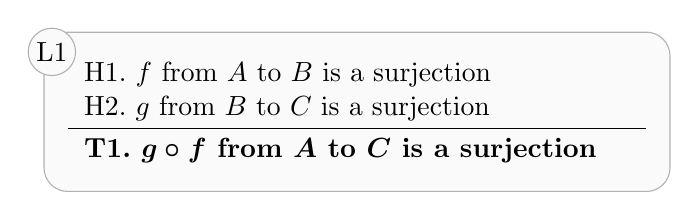
\begin{tikzpicture}[baseline=(main.base)]%
\node[tableau] (main) {%
\\

\begin{tabular}{ll}%
H1.\ $\textrm{$f$ from $A$ to $B$ is a surjection}$&\\
H2.\ $\textrm{$g$ from $B$ to $C$ is a surjection}$&
\Bstrut\\\hline\Tstrut
\textbf{\boldmath T1.\ $\textrm{$g\circ f$ from $A$ to $C$ is a surjection}$\unboldmath }&\textbf{\boldmath \unboldmath }
\end{tabular}%
};%
\node[tableaulabel] at (main.north west) [xshift=4mm, yshift=-5.5mm] {L1};
\end{tikzpicture}%
\end{fit}
\smallskip

\noindent1. Expand pre-universal target T1.\nopagebreak[4] 
\marginpar{}\nopagebreak[4] 
\smallskip\nopagebreak[4] 

\begin{fit}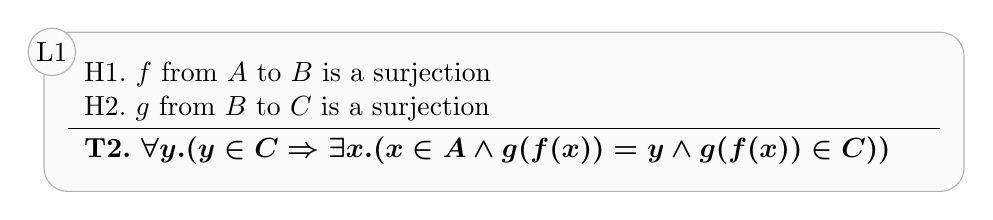
\begin{tikzpicture}[baseline=(main.base)]%
\node[tableau] (main) {%
\\

\begin{tabular}{ll}%
H1.\ $\textrm{$f$ from $A$ to $B$ is a surjection}$&\\
H2.\ $\textrm{$g$ from $B$ to $C$ is a surjection}$&
\Bstrut\\\hline\Tstrut
\textbf{\boldmath T2.\ $\forall y.(\textrm{$y\in C$}\Rightarrow \exists x.(\textrm{$x\in A$}\wedge \textrm{$g(f(x)) = y$}\wedge \textrm{$g(f(x))\in C$}))$\unboldmath }&\textbf{\boldmath \unboldmath }
\end{tabular}%
};%
\node[tableaulabel] at (main.north west) [xshift=4mm, yshift=-5.5mm] {L1};
\end{tikzpicture}%
\end{fit}
\smallskip

\noindent2. Apply `let' trick and move premise of universal-conditional target T2 above the line.\nopagebreak[4] 
\marginpar{Let $y$ be an element of $C$.}\nopagebreak[4] 
\smallskip\nopagebreak[4] 

\begin{fit}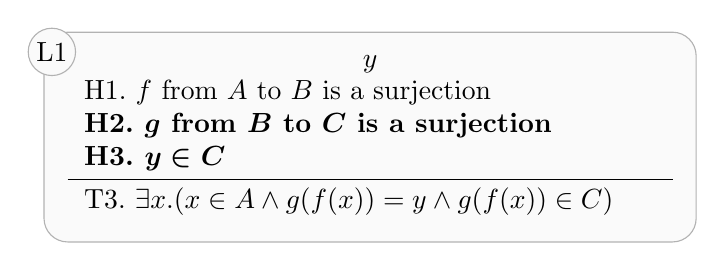
\begin{tikzpicture}[baseline=(main.base)]%
\node[tableau] (main) {%
$y$\\

\begin{tabular}{ll}%
H1.\ $\textrm{$f$ from $A$ to $B$ is a surjection}$&\\
\textbf{\boldmath H2.\ $\textrm{$g$ from $B$ to $C$ is a surjection}$\unboldmath }&\textbf{\boldmath \unboldmath }\\
\textbf{\boldmath H3.\ $\textrm{$y\in C$}$\unboldmath }&\textbf{\boldmath \unboldmath }
\Bstrut\\\hline\Tstrut
T3.\ $\exists x.(\textrm{$x\in A$}\wedge \textrm{$g(f(x)) = y$}\wedge \textrm{$g(f(x))\in C$})$&
\end{tabular}%
};%
\node[tableaulabel] at (main.north west) [xshift=4mm, yshift=-5.5mm] {L1};
\end{tikzpicture}%
\end{fit}
\smallskip

\noindent3. Forwards reasoning using H2 with H3.\nopagebreak[4] 
\marginpar{Since $g$ from $B$ to $C$ is a surjection and $y\in C$, there exists $u\in B$ such that $g(u) = y$ and $g(u)\in C$.}\nopagebreak[4] 
\smallskip\nopagebreak[4] 

\begin{fit}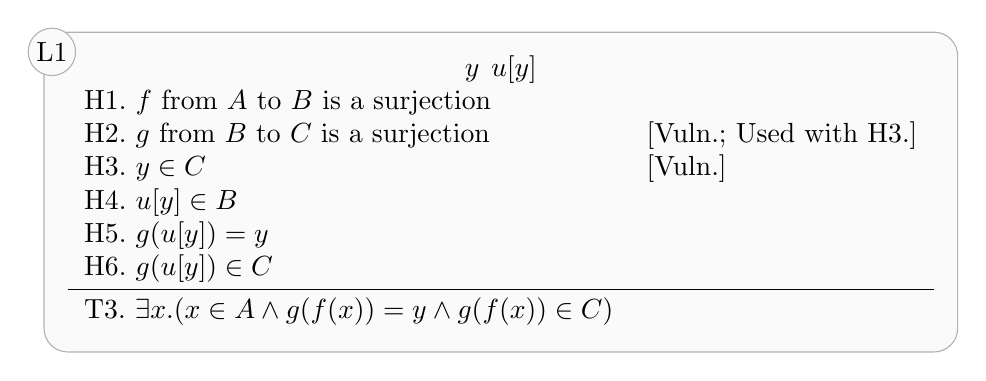
\begin{tikzpicture}[baseline=(main.base)]%
\node[tableau] (main) {%
$y$\hspace{1.5mm}$u[y]$\\

\begin{tabular}{ll}%
H1.\ $\textrm{$f$ from $A$ to $B$ is a surjection}$&\\
H2.\ $\textrm{$g$ from $B$ to $C$ is a surjection}$&[Vuln.; Used with H3.]\\
H3.\ $\textrm{$y\in C$}$&[Vuln.]\\
H4.\ $\textrm{$u[y]\in B$}$&\\
H5.\ $\textrm{$g(u[y]) = y$}$&\\
H6.\ $\textrm{$g(u[y])\in C$}$&
\Bstrut\\\hline\Tstrut
T3.\ $\exists x.(\textrm{$x\in A$}\wedge \textrm{$g(f(x)) = y$}\wedge \textrm{$g(f(x))\in C$})$&
\end{tabular}%
};%
\node[tableaulabel] at (main.north west) [xshift=4mm, yshift=-5.5mm] {L1};
\end{tikzpicture}%
\end{fit}
\smallskip

\noindent4. Deleted H3, as this unexpandable atomic statement is unmatchable.\nopagebreak[4] 
\marginpar{}\nopagebreak[4] 
\smallskip\nopagebreak[4] 

\begin{fit}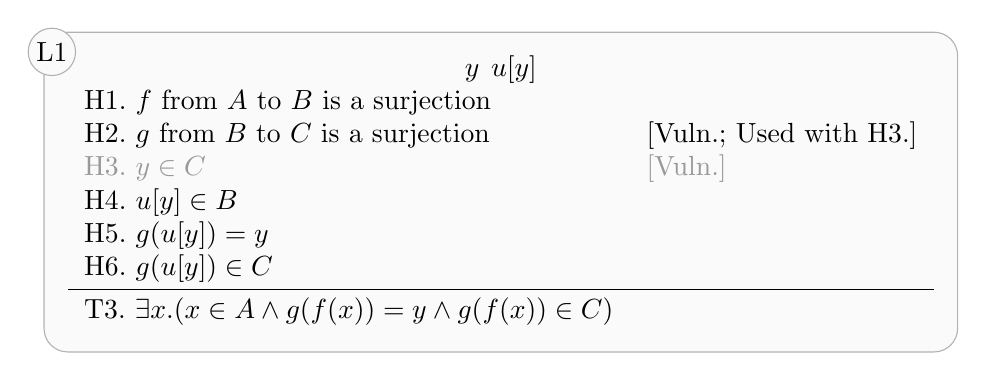
\begin{tikzpicture}[baseline=(main.base)]%
\node[tableau] (main) {%
$y$\hspace{1.5mm}$u[y]$\\

\begin{tabular}{ll}%
H1.\ $\textrm{$f$ from $A$ to $B$ is a surjection}$&\\
H2.\ $\textrm{$g$ from $B$ to $C$ is a surjection}$&[Vuln.; Used with H3.]\\
\grey{H3.\ $\textrm{$y\in C$}$}&\grey{[Vuln.]}\\
H4.\ $\textrm{$u[y]\in B$}$&\\
H5.\ $\textrm{$g(u[y]) = y$}$&\\
H6.\ $\textrm{$g(u[y])\in C$}$&
\Bstrut\\\hline\Tstrut
T3.\ $\exists x.(\textrm{$x\in A$}\wedge \textrm{$g(f(x)) = y$}\wedge \textrm{$g(f(x))\in C$})$&
\end{tabular}%
};%
\node[tableaulabel] at (main.north west) [xshift=4mm, yshift=-5.5mm] {L1};
\end{tikzpicture}%
\end{fit}
\smallskip

\noindent5. Deleted H2, as the conclusion of this implicative statement is unmatchable.\nopagebreak[4] 
\marginpar{}\nopagebreak[4] 
\smallskip\nopagebreak[4] 

\begin{fit}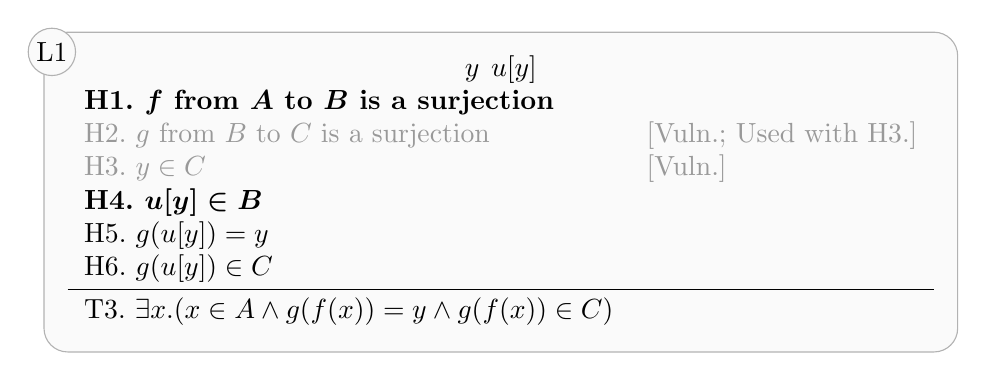
\begin{tikzpicture}[baseline=(main.base)]%
\node[tableau] (main) {%
$y$\hspace{1.5mm}$u[y]$\\

\begin{tabular}{ll}%
\textbf{\boldmath H1.\ $\textrm{$f$ from $A$ to $B$ is a surjection}$\unboldmath }&\textbf{\boldmath \unboldmath }\\
\grey{H2.\ $\textrm{$g$ from $B$ to $C$ is a surjection}$}&\grey{[Vuln.; Used with H3.]}\\
\grey{H3.\ $\textrm{$y\in C$}$}&\grey{[Vuln.]}\\
\textbf{\boldmath H4.\ $\textrm{$u[y]\in B$}$\unboldmath }&\textbf{\boldmath \unboldmath }\\
H5.\ $\textrm{$g(u[y]) = y$}$&\\
H6.\ $\textrm{$g(u[y])\in C$}$&
\Bstrut\\\hline\Tstrut
T3.\ $\exists x.(\textrm{$x\in A$}\wedge \textrm{$g(f(x)) = y$}\wedge \textrm{$g(f(x))\in C$})$&
\end{tabular}%
};%
\node[tableaulabel] at (main.north west) [xshift=4mm, yshift=-5.5mm] {L1};
\end{tikzpicture}%
\end{fit}
\smallskip

\noindent6. Forwards reasoning using H1 with H4.\nopagebreak[4] 
\marginpar{Since $f$ from $A$ to $B$ is a surjection and $u\in B$, there exists $v\in A$ such that $f(v) = u$ and $f(v)\in B$.}\nopagebreak[4] 
\smallskip\nopagebreak[4] 

\begin{fit}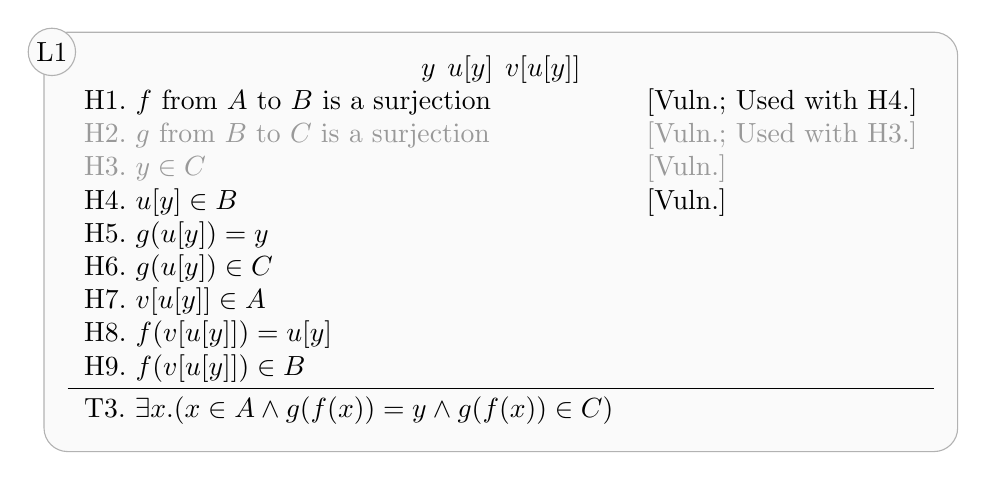
\begin{tikzpicture}[baseline=(main.base)]%
\node[tableau] (main) {%
$y$\hspace{1.5mm}$u[y]$\hspace{1.5mm}$v[u[y]]$\\

\begin{tabular}{ll}%
H1.\ $\textrm{$f$ from $A$ to $B$ is a surjection}$&[Vuln.; Used with H4.]\\
\grey{H2.\ $\textrm{$g$ from $B$ to $C$ is a surjection}$}&\grey{[Vuln.; Used with H3.]}\\
\grey{H3.\ $\textrm{$y\in C$}$}&\grey{[Vuln.]}\\
H4.\ $\textrm{$u[y]\in B$}$&[Vuln.]\\
H5.\ $\textrm{$g(u[y]) = y$}$&\\
H6.\ $\textrm{$g(u[y])\in C$}$&\\
H7.\ $\textrm{$v[u[y]]\in A$}$&\\
H8.\ $\textrm{$f(v[u[y]]) = u[y]$}$&\\
H9.\ $\textrm{$f(v[u[y]])\in B$}$&
\Bstrut\\\hline\Tstrut
T3.\ $\exists x.(\textrm{$x\in A$}\wedge \textrm{$g(f(x)) = y$}\wedge \textrm{$g(f(x))\in C$})$&
\end{tabular}%
};%
\node[tableaulabel] at (main.north west) [xshift=4mm, yshift=-5.5mm] {L1};
\end{tikzpicture}%
\end{fit}
\smallskip

\noindent7. Deleted H4, as this unexpandable atomic statement is unmatchable.\nopagebreak[4] 
\marginpar{}\nopagebreak[4] 
\smallskip\nopagebreak[4] 

\begin{fit}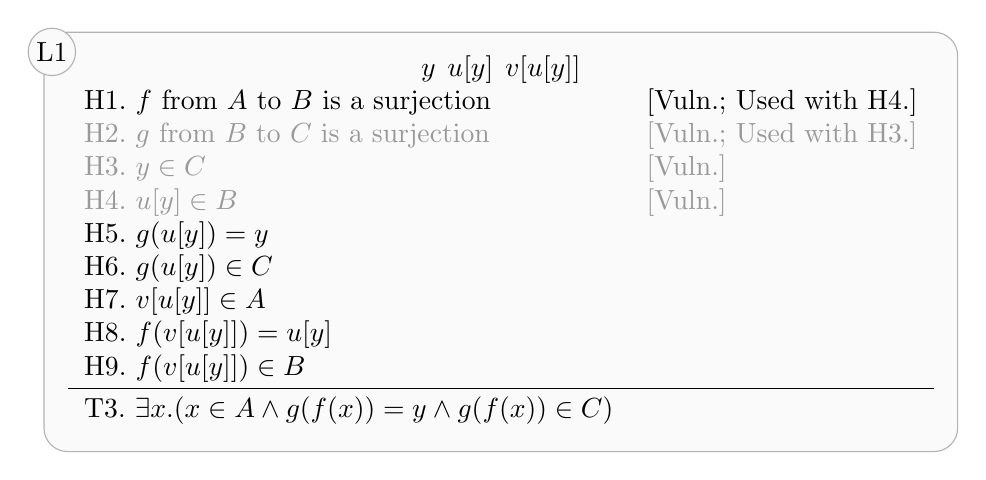
\begin{tikzpicture}[baseline=(main.base)]%
\node[tableau] (main) {%
$y$\hspace{1.5mm}$u[y]$\hspace{1.5mm}$v[u[y]]$\\

\begin{tabular}{ll}%
H1.\ $\textrm{$f$ from $A$ to $B$ is a surjection}$&[Vuln.; Used with H4.]\\
\grey{H2.\ $\textrm{$g$ from $B$ to $C$ is a surjection}$}&\grey{[Vuln.; Used with H3.]}\\
\grey{H3.\ $\textrm{$y\in C$}$}&\grey{[Vuln.]}\\
\grey{H4.\ $\textrm{$u[y]\in B$}$}&\grey{[Vuln.]}\\
H5.\ $\textrm{$g(u[y]) = y$}$&\\
H6.\ $\textrm{$g(u[y])\in C$}$&\\
H7.\ $\textrm{$v[u[y]]\in A$}$&\\
H8.\ $\textrm{$f(v[u[y]]) = u[y]$}$&\\
H9.\ $\textrm{$f(v[u[y]])\in B$}$&
\Bstrut\\\hline\Tstrut
T3.\ $\exists x.(\textrm{$x\in A$}\wedge \textrm{$g(f(x)) = y$}\wedge \textrm{$g(f(x))\in C$})$&
\end{tabular}%
};%
\node[tableaulabel] at (main.north west) [xshift=4mm, yshift=-5.5mm] {L1};
\end{tikzpicture}%
\end{fit}
\smallskip

\noindent8. Deleted H1, as the conclusion of this implicative statement is unmatchable.\nopagebreak[4] 
\marginpar{}\nopagebreak[4] 
\smallskip\nopagebreak[4] 

\begin{fit}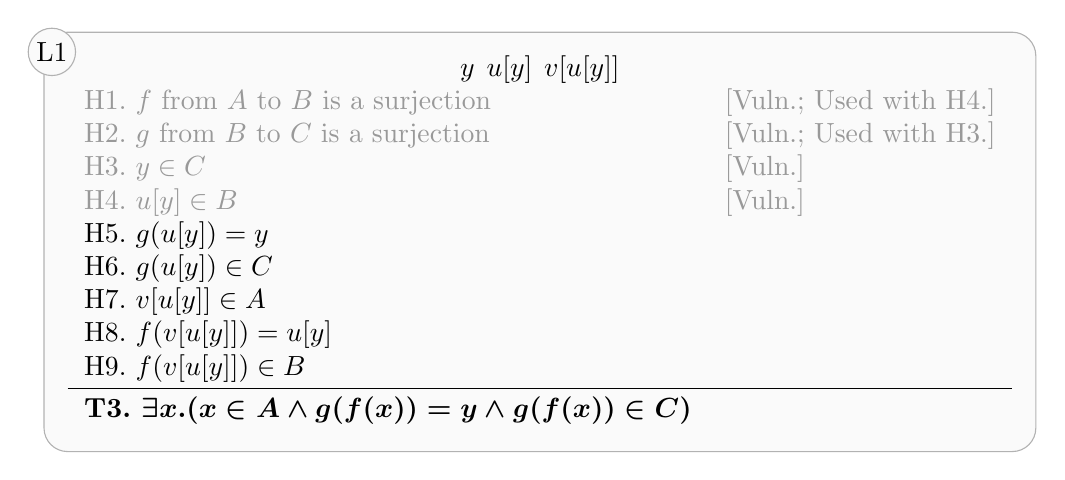
\begin{tikzpicture}[baseline=(main.base)]%
\node[tableau] (main) {%
$y$\hspace{1.5mm}$u[y]$\hspace{1.5mm}$v[u[y]]$\\

\begin{tabular}{ll}%
\grey{H1.\ $\textrm{$f$ from $A$ to $B$ is a surjection}$}&\grey{[Vuln.; Used with H4.]}\\
\grey{H2.\ $\textrm{$g$ from $B$ to $C$ is a surjection}$}&\grey{[Vuln.; Used with H3.]}\\
\grey{H3.\ $\textrm{$y\in C$}$}&\grey{[Vuln.]}\\
\grey{H4.\ $\textrm{$u[y]\in B$}$}&\grey{[Vuln.]}\\
H5.\ $\textrm{$g(u[y]) = y$}$&\\
H6.\ $\textrm{$g(u[y])\in C$}$&\\
H7.\ $\textrm{$v[u[y]]\in A$}$&\\
H8.\ $\textrm{$f(v[u[y]]) = u[y]$}$&\\
H9.\ $\textrm{$f(v[u[y]])\in B$}$&
\Bstrut\\\hline\Tstrut
\textbf{\boldmath T3.\ $\exists x.(\textrm{$x\in A$}\wedge \textrm{$g(f(x)) = y$}\wedge \textrm{$g(f(x))\in C$})$\unboldmath }&\textbf{\boldmath \unboldmath }
\end{tabular}%
};%
\node[tableaulabel] at (main.north west) [xshift=4mm, yshift=-5.5mm] {L1};
\end{tikzpicture}%
\end{fit}
\smallskip

\noindent9. Unlock existential target T3.\nopagebreak[4] 
\marginpar{We would like to find $x\in A$ s.t. $g(f(x)) = y$ and $g(f(x))\in C$.}\nopagebreak[4] 
\smallskip\nopagebreak[4] 

\begin{fit}\begin{tikzpicture}[baseline=(main.base)]%
\node[tableau] (main) {%
$y$\hspace{1.5mm}$u[y]$\hspace{1.5mm}$v[u[y]]$\\

\begin{tabular}{ll}%
\grey{H1.\ $\textrm{$f$ from $A$ to $B$ is a surjection}$}&\grey{[Vuln.; Used with H4.]}\\
\grey{H2.\ $\textrm{$g$ from $B$ to $C$ is a surjection}$}&\grey{[Vuln.; Used with H3.]}\\
\grey{H3.\ $\textrm{$y\in C$}$}&\grey{[Vuln.]}\\
\grey{H4.\ $\textrm{$u[y]\in B$}$}&\grey{[Vuln.]}\\
H5.\ $\textrm{$g(u[y]) = y$}$&\\
H6.\ $\textrm{$g(u[y])\in C$}$&\\
H7.\ $\textrm{$v[u[y]]\in A$}$&\\
H8.\ $\textrm{$f(v[u[y]]) = u[y]$}$&\\
H9.\ $\textrm{$f(v[u[y]])\in B$}$&
\Bstrut\\\hline\Tstrut
\begin{tikzpicture}[baseline=(main.base)]%
\node[tableau] (main) {%
$x^\blacklozenge $\\

\begin{tabular}{ll}%

\Bstrut\\\hline\Tstrut
T4.\ $\textrm{$x^\blacklozenge \in A$}$&\\
T5.\ $\textrm{$g(f(x^\blacklozenge )) = y$}$&\\
T6.\ $\textrm{$g(f(x^\blacklozenge ))\in C$}$&
\end{tabular}%
};%
\node[tableaulabel] at (main.north west) [xshift=4mm, yshift=-5.5mm] {L2$^\blacklozenge$};
\end{tikzpicture}%

\end{tabular}%
};%
\node[tableaulabel] at (main.north west) [xshift=4mm, yshift=-5.5mm] {L1};
\end{tikzpicture}%
\end{fit}

No moves possible.
\cleardoublepage

\end{steps}
{\begin{center} \large \textbf{If $f$ is a surjection then $f(A)^c \subset f(A^c)$}\end{center}}\nopagebreak[4]

\begin{center}
\begin{minipage}{120mm}
Let $x$ be an element of $(f(A))^c$. Then $x\notin f(A)$. Then it is not that case that $x\in f(A)$. We would like to find $y\in (A)^c$ s.t. $f(y) = x$. But $y\in (A)^c$ if and only if $y\notin A$. But $y\notin A$ if and only if it is not that case that $y\in A$.
\end{minipage}
\end{center}

\bigskip
\begin{steps}
\begin{fit}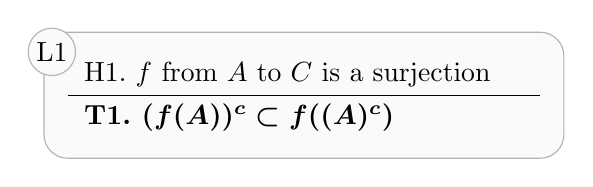
\begin{tikzpicture}[baseline=(main.base)]%
\node[tableau] (main) {%
\\

\begin{tabular}{ll}%
H1.\ $\textrm{$f$ from $A$ to $C$ is a surjection}$&
\Bstrut\\\hline\Tstrut
\textbf{\boldmath T1.\ $\textrm{$(f(A))^c\subset f((A)^c)$}$\unboldmath }&\textbf{\boldmath \unboldmath }
\end{tabular}%
};%
\node[tableaulabel] at (main.north west) [xshift=4mm, yshift=-5.5mm] {L1};
\end{tikzpicture}%
\end{fit}
\smallskip

\noindent1. Expand pre-universal target T1.\nopagebreak[4] 
\marginpar{}\nopagebreak[4] 
\smallskip\nopagebreak[4] 

\begin{fit}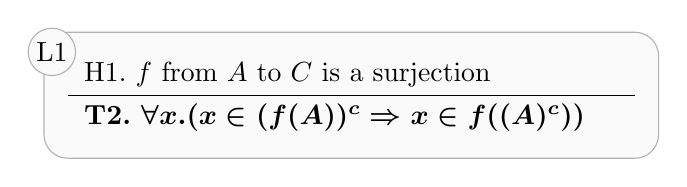
\begin{tikzpicture}[baseline=(main.base)]%
\node[tableau] (main) {%
\\

\begin{tabular}{ll}%
H1.\ $\textrm{$f$ from $A$ to $C$ is a surjection}$&
\Bstrut\\\hline\Tstrut
\textbf{\boldmath T2.\ $\forall x.(\textrm{$x\in (f(A))^c$}\Rightarrow \textrm{$x\in f((A)^c)$})$\unboldmath }&\textbf{\boldmath \unboldmath }
\end{tabular}%
};%
\node[tableaulabel] at (main.north west) [xshift=4mm, yshift=-5.5mm] {L1};
\end{tikzpicture}%
\end{fit}
\smallskip

\noindent2. Apply `let' trick and move premise of universal-conditional target T2 above the line.\nopagebreak[4] 
\marginpar{Let $x$ be an element of $(f(A))^c$.}\nopagebreak[4] 
\smallskip\nopagebreak[4] 

\begin{fit}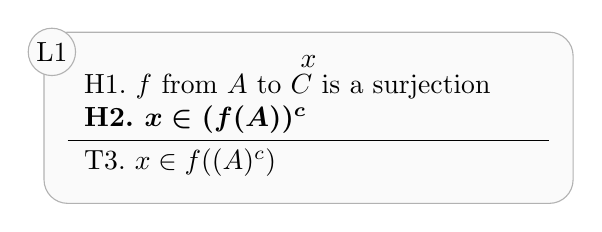
\begin{tikzpicture}[baseline=(main.base)]%
\node[tableau] (main) {%
$x$\\

\begin{tabular}{ll}%
H1.\ $\textrm{$f$ from $A$ to $C$ is a surjection}$&\\
\textbf{\boldmath H2.\ $\textrm{$x\in (f(A))^c$}$\unboldmath }&\textbf{\boldmath \unboldmath }
\Bstrut\\\hline\Tstrut
T3.\ $\textrm{$x\in f((A)^c)$}$&
\end{tabular}%
};%
\node[tableaulabel] at (main.north west) [xshift=4mm, yshift=-5.5mm] {L1};
\end{tikzpicture}%
\end{fit}
\smallskip

\noindent3. Quantifier-free expansion of hypothesis H2.\nopagebreak[4] 
\marginpar{Since $x\in (f(A))^c$, we have that $x\notin f(A)$.}\nopagebreak[4] 
\smallskip\nopagebreak[4] 

\begin{fit}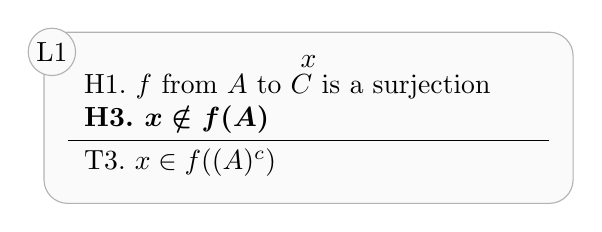
\begin{tikzpicture}[baseline=(main.base)]%
\node[tableau] (main) {%
$x$\\

\begin{tabular}{ll}%
H1.\ $\textrm{$f$ from $A$ to $C$ is a surjection}$&\\
\textbf{\boldmath H3.\ $\textrm{$x\notin f(A)$}$\unboldmath }&\textbf{\boldmath \unboldmath }
\Bstrut\\\hline\Tstrut
T3.\ $\textrm{$x\in f((A)^c)$}$&
\end{tabular}%
};%
\node[tableaulabel] at (main.north west) [xshift=4mm, yshift=-5.5mm] {L1};
\end{tikzpicture}%
\end{fit}
\smallskip

\noindent4. Quantifier-free expansion of hypothesis H3.\nopagebreak[4] 
\marginpar{Since $x\notin f(A)$, it is not that case that $x\in f(A)$.}\nopagebreak[4] 
\smallskip\nopagebreak[4] 

\begin{fit}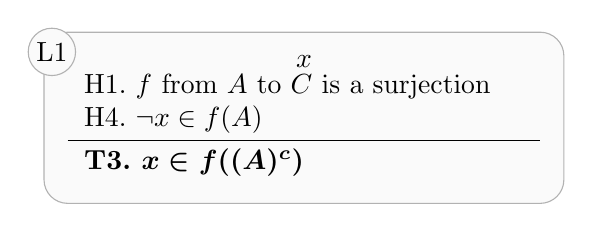
\begin{tikzpicture}[baseline=(main.base)]%
\node[tableau] (main) {%
$x$\\

\begin{tabular}{ll}%
H1.\ $\textrm{$f$ from $A$ to $C$ is a surjection}$&\\
H4.\ $\neg \textrm{$x\in f(A)$}$&
\Bstrut\\\hline\Tstrut
\textbf{\boldmath T3.\ $\textrm{$x\in f((A)^c)$}$\unboldmath }&\textbf{\boldmath \unboldmath }
\end{tabular}%
};%
\node[tableaulabel] at (main.north west) [xshift=4mm, yshift=-5.5mm] {L1};
\end{tikzpicture}%
\end{fit}
\smallskip

\noindent5. Expand pre-existential target T3.\nopagebreak[4] 
\marginpar{We would like to find $y\in (A)^c$ s.t. $f(y) = x$.}\nopagebreak[4] 
\smallskip\nopagebreak[4] 

\begin{fit}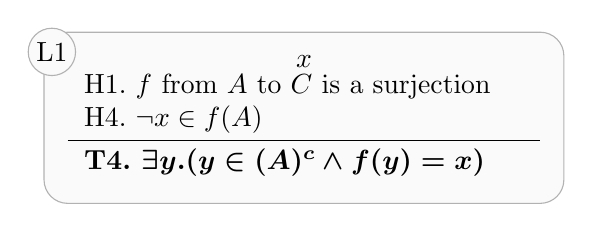
\begin{tikzpicture}[baseline=(main.base)]%
\node[tableau] (main) {%
$x$\\

\begin{tabular}{ll}%
H1.\ $\textrm{$f$ from $A$ to $C$ is a surjection}$&\\
H4.\ $\neg \textrm{$x\in f(A)$}$&
\Bstrut\\\hline\Tstrut
\textbf{\boldmath T4.\ $\exists y.(\textrm{$y\in (A)^c$}\wedge \textrm{$f(y) = x$})$\unboldmath }&\textbf{\boldmath \unboldmath }
\end{tabular}%
};%
\node[tableaulabel] at (main.north west) [xshift=4mm, yshift=-5.5mm] {L1};
\end{tikzpicture}%
\end{fit}
\smallskip

\noindent6. Unlock existential target T4.\nopagebreak[4] 
\marginpar{We would like to find $y\in (A)^c$ s.t. $f(y) = x$.}\nopagebreak[4] 
\smallskip\nopagebreak[4] 

\begin{fit}\begin{tikzpicture}[baseline=(main.base)]%
\node[tableau] (main) {%
$x$\\

\begin{tabular}{ll}%
H1.\ $\textrm{$f$ from $A$ to $C$ is a surjection}$&\\
H4.\ $\neg \textrm{$x\in f(A)$}$&
\Bstrut\\\hline\Tstrut
\begin{tikzpicture}[baseline=(main.base)]%
\node[tableau] (main) {%
$y^\blacklozenge $\\

\begin{tabular}{ll}%

\Bstrut\\\hline\Tstrut
\textbf{\boldmath T5.\ $\textrm{$y^\blacklozenge \in (A)^c$}$\unboldmath }&\textbf{\boldmath \unboldmath }\\
T6.\ $\textrm{$f(y^\blacklozenge ) = x$}$&
\end{tabular}%
};%
\node[tableaulabel] at (main.north west) [xshift=4mm, yshift=-5.5mm] {L2$^\blacklozenge$};
\end{tikzpicture}%

\end{tabular}%
};%
\node[tableaulabel] at (main.north west) [xshift=4mm, yshift=-5.5mm] {L1};
\end{tikzpicture}%
\end{fit}
\smallskip

\noindent7. Quantifier-free expansion of target T5.\nopagebreak[4] 
\marginpar{But $y\in (A)^c$ if and only if $y\notin A$.}\nopagebreak[4] 
\smallskip\nopagebreak[4] 

\begin{fit}\begin{tikzpicture}[baseline=(main.base)]%
\node[tableau] (main) {%
$x$\\

\begin{tabular}{ll}%
H1.\ $\textrm{$f$ from $A$ to $C$ is a surjection}$&\\
H4.\ $\neg \textrm{$x\in f(A)$}$&
\Bstrut\\\hline\Tstrut
\begin{tikzpicture}[baseline=(main.base)]%
\node[tableau] (main) {%
$y^\blacklozenge $\\

\begin{tabular}{ll}%

\Bstrut\\\hline\Tstrut
\textbf{\boldmath T7.\ $\textrm{$y^\blacklozenge \notin A$}$\unboldmath }&\textbf{\boldmath \unboldmath }\\
T6.\ $\textrm{$f(y^\blacklozenge ) = x$}$&
\end{tabular}%
};%
\node[tableaulabel] at (main.north west) [xshift=4mm, yshift=-5.5mm] {L2$^\blacklozenge$};
\end{tikzpicture}%

\end{tabular}%
};%
\node[tableaulabel] at (main.north west) [xshift=4mm, yshift=-5.5mm] {L1};
\end{tikzpicture}%
\end{fit}
\smallskip

\noindent8. Quantifier-free expansion of target T7.\nopagebreak[4] 
\marginpar{But $y\notin A$ if and only if it is not that case that $y\in A$.}\nopagebreak[4] 
\smallskip\nopagebreak[4] 

\begin{fit}\begin{tikzpicture}[baseline=(main.base)]%
\node[tableau] (main) {%
$x$\\

\begin{tabular}{ll}%
H1.\ $\textrm{$f$ from $A$ to $C$ is a surjection}$&\\
H4.\ $\neg \textrm{$x\in f(A)$}$&
\Bstrut\\\hline\Tstrut
\begin{tikzpicture}[baseline=(main.base)]%
\node[tableau] (main) {%
$y^\blacklozenge $\\

\begin{tabular}{ll}%

\Bstrut\\\hline\Tstrut
T8.\ $\neg \textrm{$y^\blacklozenge \in A$}$&\\
T6.\ $\textrm{$f(y^\blacklozenge ) = x$}$&
\end{tabular}%
};%
\node[tableaulabel] at (main.north west) [xshift=4mm, yshift=-5.5mm] {L2$^\blacklozenge$};
\end{tikzpicture}%

\end{tabular}%
};%
\node[tableaulabel] at (main.north west) [xshift=4mm, yshift=-5.5mm] {L1};
\end{tikzpicture}%
\end{fit}

No moves possible.
\cleardoublepage

\end{steps}
{\begin{center} \large \textbf{Prove that $(A \cap B)^c \subset A^c \cup B^c$}\end{center}}\nopagebreak[4]

\begin{center}
\begin{minipage}{120mm}
Let $x$ be an element of $(A\cap B)^c$. Then $x\notin A\cap B$. Then it is not that case that $x\in A\cap B$. We would like to show that $x\in (A)^c\cup (B)^c$, i.e. that $x\in (A)^c$ or $x\in (B)^c$. We would like to show that $x\in (A)^c$, i.e. that $x\notin A$. We would like to show that $x\notin A$, i.e. that it is not that case that $x\in A$. We would like to show that $x\in (B)^c$, i.e. that $x\notin B$. We would like to show that $x\notin B$, i.e. that it is not that case that $x\in B$.
\end{minipage}
\end{center}

\bigskip
\begin{steps}
\begin{fit}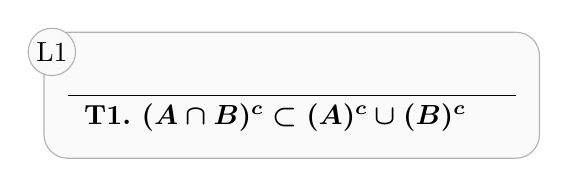
\begin{tikzpicture}[baseline=(main.base)]%
\node[tableau] (main) {%
\\

\begin{tabular}{ll}%

\Bstrut\\\hline\Tstrut
\textbf{\boldmath T1.\ $\textrm{$(A\cap B)^c\subset (A)^c\cup (B)^c$}$\unboldmath }&\textbf{\boldmath \unboldmath }
\end{tabular}%
};%
\node[tableaulabel] at (main.north west) [xshift=4mm, yshift=-5.5mm] {L1};
\end{tikzpicture}%
\end{fit}
\smallskip

\noindent1. Expand pre-universal target T1.\nopagebreak[4] 
\marginpar{}\nopagebreak[4] 
\smallskip\nopagebreak[4] 

\begin{fit}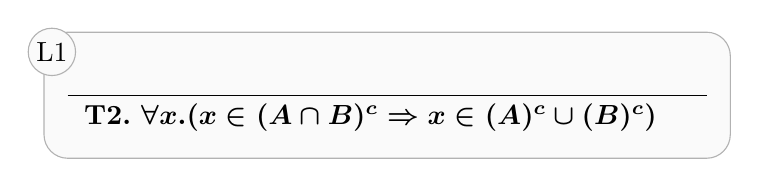
\begin{tikzpicture}[baseline=(main.base)]%
\node[tableau] (main) {%
\\

\begin{tabular}{ll}%

\Bstrut\\\hline\Tstrut
\textbf{\boldmath T2.\ $\forall x.(\textrm{$x\in (A\cap B)^c$}\Rightarrow \textrm{$x\in (A)^c\cup (B)^c$})$\unboldmath }&\textbf{\boldmath \unboldmath }
\end{tabular}%
};%
\node[tableaulabel] at (main.north west) [xshift=4mm, yshift=-5.5mm] {L1};
\end{tikzpicture}%
\end{fit}
\smallskip

\noindent2. Apply `let' trick and move premise of universal-conditional target T2 above the line.\nopagebreak[4] 
\marginpar{Let $x$ be an element of $(A\cap B)^c$.}\nopagebreak[4] 
\smallskip\nopagebreak[4] 

\begin{fit}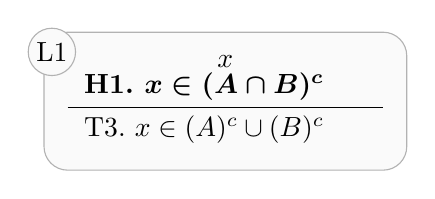
\begin{tikzpicture}[baseline=(main.base)]%
\node[tableau] (main) {%
$x$\\

\begin{tabular}{ll}%
\textbf{\boldmath H1.\ $\textrm{$x\in (A\cap B)^c$}$\unboldmath }&\textbf{\boldmath \unboldmath }
\Bstrut\\\hline\Tstrut
T3.\ $\textrm{$x\in (A)^c\cup (B)^c$}$&
\end{tabular}%
};%
\node[tableaulabel] at (main.north west) [xshift=4mm, yshift=-5.5mm] {L1};
\end{tikzpicture}%
\end{fit}
\smallskip

\noindent3. Quantifier-free expansion of hypothesis H1.\nopagebreak[4] 
\marginpar{Since $x\in (A\cap B)^c$, we have that $x\notin A\cap B$.}\nopagebreak[4] 
\smallskip\nopagebreak[4] 

\begin{fit}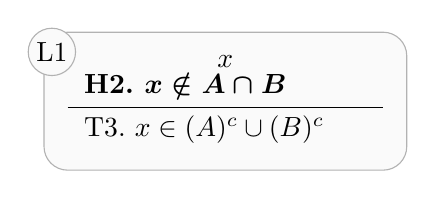
\begin{tikzpicture}[baseline=(main.base)]%
\node[tableau] (main) {%
$x$\\

\begin{tabular}{ll}%
\textbf{\boldmath H2.\ $\textrm{$x\notin A\cap B$}$\unboldmath }&\textbf{\boldmath \unboldmath }
\Bstrut\\\hline\Tstrut
T3.\ $\textrm{$x\in (A)^c\cup (B)^c$}$&
\end{tabular}%
};%
\node[tableaulabel] at (main.north west) [xshift=4mm, yshift=-5.5mm] {L1};
\end{tikzpicture}%
\end{fit}
\smallskip

\noindent4. Quantifier-free expansion of hypothesis H2.\nopagebreak[4] 
\marginpar{Since $x\notin A\cap B$, it is not that case that $x\in A\cap B$.}\nopagebreak[4] 
\smallskip\nopagebreak[4] 

\begin{fit}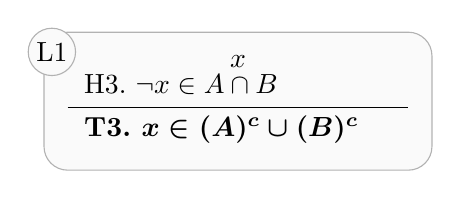
\begin{tikzpicture}[baseline=(main.base)]%
\node[tableau] (main) {%
$x$\\

\begin{tabular}{ll}%
H3.\ $\neg \textrm{$x\in A\cap B$}$&
\Bstrut\\\hline\Tstrut
\textbf{\boldmath T3.\ $\textrm{$x\in (A)^c\cup (B)^c$}$\unboldmath }&\textbf{\boldmath \unboldmath }
\end{tabular}%
};%
\node[tableaulabel] at (main.north west) [xshift=4mm, yshift=-5.5mm] {L1};
\end{tikzpicture}%
\end{fit}
\smallskip

\noindent5. Quantifier-free expansion of target T3.\nopagebreak[4] 
\marginpar{We would like to show that $x\in (A)^c\cup (B)^c$, i.e. that $x\in (A)^c$ or $x\in (B)^c$.}\nopagebreak[4] 
\smallskip\nopagebreak[4] 

\begin{fit}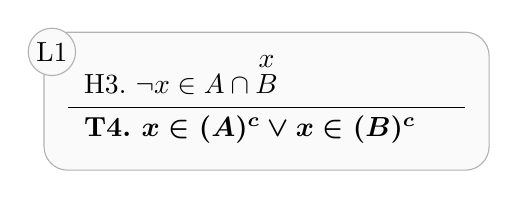
\begin{tikzpicture}[baseline=(main.base)]%
\node[tableau] (main) {%
$x$\\

\begin{tabular}{ll}%
H3.\ $\neg \textrm{$x\in A\cap B$}$&
\Bstrut\\\hline\Tstrut
\textbf{\boldmath T4.\ $\textrm{$x\in (A)^c$}\vee \textrm{$x\in (B)^c$}$\unboldmath }&\textbf{\boldmath \unboldmath }
\end{tabular}%
};%
\node[tableaulabel] at (main.north west) [xshift=4mm, yshift=-5.5mm] {L1};
\end{tikzpicture}%
\end{fit}
\smallskip

\noindent6. Split up disjunctive target T4.\nopagebreak[4] 
\marginpar{}\nopagebreak[4] 
\smallskip\nopagebreak[4] 

\begin{fit}\begin{tikzpicture}[baseline=(main.base)]%
\node[tableau] (main) {%
$x$\\

\begin{tabular}{ll}%
H3.\ $\neg \textrm{$x\in A\cap B$}$&
\Bstrut\\\hline\Tstrut
\begin{tikzpicture}[baseline=(main.base)]%
\node[tableau] (main) {%
\\

\begin{tabular}{ll}%

\Bstrut\\\hline\Tstrut
\textbf{\boldmath T7.\ $\textrm{$x\in (A)^c$}$\unboldmath }&\textbf{\boldmath \unboldmath }
\end{tabular}%
};%
\node[tableaulabel] at (main.north west) [xshift=4mm, yshift=-5.5mm] {L4};
\end{tikzpicture}%
\hspace{2mm}$\vee$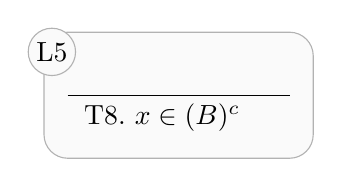
\begin{tikzpicture}[baseline=(main.base)]%
\node[tableau] (main) {%
\\

\begin{tabular}{ll}%

\Bstrut\\\hline\Tstrut
T8.\ $\textrm{$x\in (B)^c$}$&
\end{tabular}%
};%
\node[tableaulabel] at (main.north west) [xshift=4mm, yshift=-5.5mm] {L5};
\end{tikzpicture}%

\end{tabular}%
};%
\node[tableaulabel] at (main.north west) [xshift=4mm, yshift=-5.5mm] {L1};
\end{tikzpicture}%
\end{fit}
\smallskip

\noindent7. Quantifier-free expansion of target T7.\nopagebreak[4] 
\marginpar{We would like to show that $x\in (A)^c$, i.e. that $x\notin A$.}\nopagebreak[4] 
\smallskip\nopagebreak[4] 

\begin{fit}\begin{tikzpicture}[baseline=(main.base)]%
\node[tableau] (main) {%
$x$\\

\begin{tabular}{ll}%
H3.\ $\neg \textrm{$x\in A\cap B$}$&
\Bstrut\\\hline\Tstrut
\begin{tikzpicture}[baseline=(main.base)]%
\node[tableau] (main) {%
\\

\begin{tabular}{ll}%

\Bstrut\\\hline\Tstrut
\textbf{\boldmath T9.\ $\textrm{$x\notin A$}$\unboldmath }&\textbf{\boldmath \unboldmath }
\end{tabular}%
};%
\node[tableaulabel] at (main.north west) [xshift=4mm, yshift=-5.5mm] {L4};
\end{tikzpicture}%
\hspace{2mm}$\vee$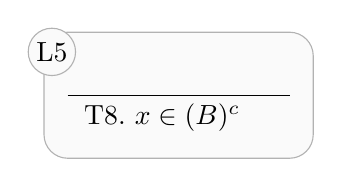
\begin{tikzpicture}[baseline=(main.base)]%
\node[tableau] (main) {%
\\

\begin{tabular}{ll}%

\Bstrut\\\hline\Tstrut
T8.\ $\textrm{$x\in (B)^c$}$&
\end{tabular}%
};%
\node[tableaulabel] at (main.north west) [xshift=4mm, yshift=-5.5mm] {L5};
\end{tikzpicture}%

\end{tabular}%
};%
\node[tableaulabel] at (main.north west) [xshift=4mm, yshift=-5.5mm] {L1};
\end{tikzpicture}%
\end{fit}
\smallskip

\noindent8. Quantifier-free expansion of target T9.\nopagebreak[4] 
\marginpar{We would like to show that $x\notin A$, i.e. that it is not that case that $x\in A$.}\nopagebreak[4] 
\smallskip\nopagebreak[4] 

\begin{fit}\begin{tikzpicture}[baseline=(main.base)]%
\node[tableau] (main) {%
$x$\\

\begin{tabular}{ll}%
H3.\ $\neg \textrm{$x\in A\cap B$}$&
\Bstrut\\\hline\Tstrut
\begin{tikzpicture}[baseline=(main.base)]%
\node[tableau] (main) {%
\\

\begin{tabular}{ll}%

\Bstrut\\\hline\Tstrut
T10.\ $\neg \textrm{$x\in A$}$&
\end{tabular}%
};%
\node[tableaulabel] at (main.north west) [xshift=4mm, yshift=-5.5mm] {L4};
\end{tikzpicture}%
\hspace{2mm}$\vee$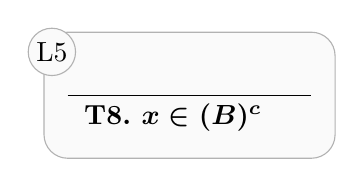
\begin{tikzpicture}[baseline=(main.base)]%
\node[tableau] (main) {%
\\

\begin{tabular}{ll}%

\Bstrut\\\hline\Tstrut
\textbf{\boldmath T8.\ $\textrm{$x\in (B)^c$}$\unboldmath }&\textbf{\boldmath \unboldmath }
\end{tabular}%
};%
\node[tableaulabel] at (main.north west) [xshift=4mm, yshift=-5.5mm] {L5};
\end{tikzpicture}%

\end{tabular}%
};%
\node[tableaulabel] at (main.north west) [xshift=4mm, yshift=-5.5mm] {L1};
\end{tikzpicture}%
\end{fit}
\smallskip

\noindent9. Quantifier-free expansion of target T8.\nopagebreak[4] 
\marginpar{We would like to show that $x\in (B)^c$, i.e. that $x\notin B$.}\nopagebreak[4] 
\smallskip\nopagebreak[4] 

\begin{fit}\begin{tikzpicture}[baseline=(main.base)]%
\node[tableau] (main) {%
$x$\\

\begin{tabular}{ll}%
H3.\ $\neg \textrm{$x\in A\cap B$}$&
\Bstrut\\\hline\Tstrut
\begin{tikzpicture}[baseline=(main.base)]%
\node[tableau] (main) {%
\\

\begin{tabular}{ll}%

\Bstrut\\\hline\Tstrut
T10.\ $\neg \textrm{$x\in A$}$&
\end{tabular}%
};%
\node[tableaulabel] at (main.north west) [xshift=4mm, yshift=-5.5mm] {L4};
\end{tikzpicture}%
\hspace{2mm}$\vee$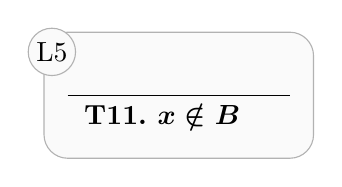
\begin{tikzpicture}[baseline=(main.base)]%
\node[tableau] (main) {%
\\

\begin{tabular}{ll}%

\Bstrut\\\hline\Tstrut
\textbf{\boldmath T11.\ $\textrm{$x\notin B$}$\unboldmath }&\textbf{\boldmath \unboldmath }
\end{tabular}%
};%
\node[tableaulabel] at (main.north west) [xshift=4mm, yshift=-5.5mm] {L5};
\end{tikzpicture}%

\end{tabular}%
};%
\node[tableaulabel] at (main.north west) [xshift=4mm, yshift=-5.5mm] {L1};
\end{tikzpicture}%
\end{fit}
\smallskip

\noindent10. Quantifier-free expansion of target T11.\nopagebreak[4] 
\marginpar{We would like to show that $x\notin B$, i.e. that it is not that case that $x\in B$.}\nopagebreak[4] 
\smallskip\nopagebreak[4] 

\begin{fit}\begin{tikzpicture}[baseline=(main.base)]%
\node[tableau] (main) {%
$x$\\

\begin{tabular}{ll}%
H3.\ $\neg \textrm{$x\in A\cap B$}$&
\Bstrut\\\hline\Tstrut
\begin{tikzpicture}[baseline=(main.base)]%
\node[tableau] (main) {%
\\

\begin{tabular}{ll}%

\Bstrut\\\hline\Tstrut
T10.\ $\neg \textrm{$x\in A$}$&
\end{tabular}%
};%
\node[tableaulabel] at (main.north west) [xshift=4mm, yshift=-5.5mm] {L4};
\end{tikzpicture}%
\hspace{2mm}$\vee$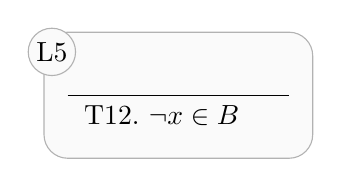
\begin{tikzpicture}[baseline=(main.base)]%
\node[tableau] (main) {%
\\

\begin{tabular}{ll}%

\Bstrut\\\hline\Tstrut
T12.\ $\neg \textrm{$x\in B$}$&
\end{tabular}%
};%
\node[tableaulabel] at (main.north west) [xshift=4mm, yshift=-5.5mm] {L5};
\end{tikzpicture}%

\end{tabular}%
};%
\node[tableaulabel] at (main.north west) [xshift=4mm, yshift=-5.5mm] {L1};
\end{tikzpicture}%
\end{fit}

No moves possible.
\cleardoublepage

\end{steps}
{\begin{center} \large \textbf{Prove that $A^c \cup B^c \subset (A \cap B)^c $}\end{center}}\nopagebreak[4]

\begin{center}
\begin{minipage}{120mm}
Let $x$ be an element of $(A)^c\cup (B)^c$. Then $x\in (A)^c$ or $x\in (B)^c$. Since $x\in (A)^c$, we have that $x\notin A$. Then it is not that case that $x\in A$. Since $x\in (B)^c$, we have that $x\notin B$. Then it is not that case that $x\in B$. We would like to show that $x\in (A\cap B)^c$, i.e. that $x\notin A\cap B$. We would like to show that $x\notin A\cap B$, i.e. that it is not that case that $x\in A\cap B$. We would like to show that $x\in (A\cap B)^c$, i.e. that $x\notin A\cap B$. We would like to show that $x\notin A\cap B$, i.e. that it is not that case that $x\in A\cap B$.
\end{minipage}
\end{center}

\bigskip
\begin{steps}
\begin{fit}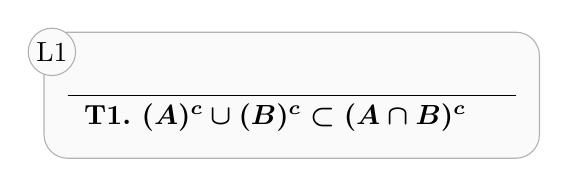
\begin{tikzpicture}[baseline=(main.base)]%
\node[tableau] (main) {%
\\

\begin{tabular}{ll}%

\Bstrut\\\hline\Tstrut
\textbf{\boldmath T1.\ $\textrm{$(A)^c\cup (B)^c\subset (A\cap B)^c$}$\unboldmath }&\textbf{\boldmath \unboldmath }
\end{tabular}%
};%
\node[tableaulabel] at (main.north west) [xshift=4mm, yshift=-5.5mm] {L1};
\end{tikzpicture}%
\end{fit}
\smallskip

\noindent1. Expand pre-universal target T1.\nopagebreak[4] 
\marginpar{}\nopagebreak[4] 
\smallskip\nopagebreak[4] 

\begin{fit}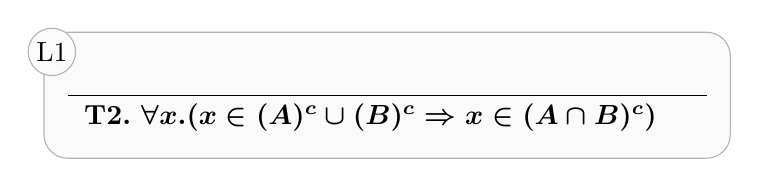
\begin{tikzpicture}[baseline=(main.base)]%
\node[tableau] (main) {%
\\

\begin{tabular}{ll}%

\Bstrut\\\hline\Tstrut
\textbf{\boldmath T2.\ $\forall x.(\textrm{$x\in (A)^c\cup (B)^c$}\Rightarrow \textrm{$x\in (A\cap B)^c$})$\unboldmath }&\textbf{\boldmath \unboldmath }
\end{tabular}%
};%
\node[tableaulabel] at (main.north west) [xshift=4mm, yshift=-5.5mm] {L1};
\end{tikzpicture}%
\end{fit}
\smallskip

\noindent2. Apply `let' trick and move premise of universal-conditional target T2 above the line.\nopagebreak[4] 
\marginpar{Let $x$ be an element of $(A)^c\cup (B)^c$.}\nopagebreak[4] 
\smallskip\nopagebreak[4] 

\begin{fit}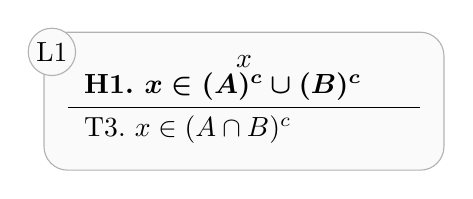
\begin{tikzpicture}[baseline=(main.base)]%
\node[tableau] (main) {%
$x$\\

\begin{tabular}{ll}%
\textbf{\boldmath H1.\ $\textrm{$x\in (A)^c\cup (B)^c$}$\unboldmath }&\textbf{\boldmath \unboldmath }
\Bstrut\\\hline\Tstrut
T3.\ $\textrm{$x\in (A\cap B)^c$}$&
\end{tabular}%
};%
\node[tableaulabel] at (main.north west) [xshift=4mm, yshift=-5.5mm] {L1};
\end{tikzpicture}%
\end{fit}
\smallskip

\noindent3. Quantifier-free expansion of hypothesis H1.\nopagebreak[4] 
\marginpar{Since $x\in (A)^c\cup (B)^c$, $x\in (A)^c$ or $x\in (B)^c$.}\nopagebreak[4] 
\smallskip\nopagebreak[4] 

\begin{fit}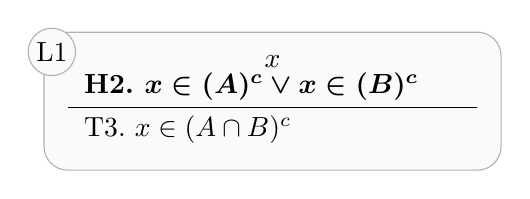
\begin{tikzpicture}[baseline=(main.base)]%
\node[tableau] (main) {%
$x$\\

\begin{tabular}{ll}%
\textbf{\boldmath H2.\ $\textrm{$x\in (A)^c$}\vee \textrm{$x\in (B)^c$}$\unboldmath }&\textbf{\boldmath \unboldmath }
\Bstrut\\\hline\Tstrut
T3.\ $\textrm{$x\in (A\cap B)^c$}$&
\end{tabular}%
};%
\node[tableaulabel] at (main.north west) [xshift=4mm, yshift=-5.5mm] {L1};
\end{tikzpicture}%
\end{fit}
\smallskip

\noindent4. Split into cases to handle disjunctive hypothesis H2.\nopagebreak[4] 
\marginpar{}\nopagebreak[4] 
\smallskip\nopagebreak[4] 

\begin{fit}\begin{tikzpicture}[baseline=(main.base)]%
\node[tableau] (main) {%
$x$\\

\begin{tabular}{ll}%

\Bstrut\\\hline\Tstrut
\begin{tikzpicture}[baseline=(main.base)]%
\node[tableau] (main) {%
\\

\begin{tabular}{ll}%
\textbf{\boldmath H3.\ $\textrm{$x\in (A)^c$}$\unboldmath }&\textbf{\boldmath \unboldmath }
\Bstrut\\\hline\Tstrut
T4.\ $\textrm{$x\in (A\cap B)^c$}$&
\end{tabular}%
};%
\node[tableaulabel] at (main.north west) [xshift=4mm, yshift=-5.5mm] {L2};
\end{tikzpicture}%
\\
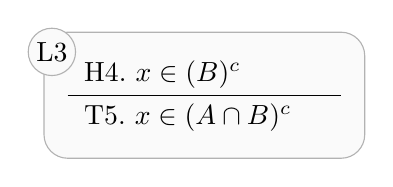
\begin{tikzpicture}[baseline=(main.base)]%
\node[tableau] (main) {%
\\

\begin{tabular}{ll}%
H4.\ $\textrm{$x\in (B)^c$}$&
\Bstrut\\\hline\Tstrut
T5.\ $\textrm{$x\in (A\cap B)^c$}$&
\end{tabular}%
};%
\node[tableaulabel] at (main.north west) [xshift=4mm, yshift=-5.5mm] {L3};
\end{tikzpicture}%

\end{tabular}%
};%
\node[tableaulabel] at (main.north west) [xshift=4mm, yshift=-5.5mm] {L1};
\end{tikzpicture}%
\end{fit}
\smallskip

\noindent5. Quantifier-free expansion of hypothesis H3.\nopagebreak[4] 
\marginpar{Since $x\in (A)^c$, we have that $x\notin A$.}\nopagebreak[4] 
\smallskip\nopagebreak[4] 

\begin{fit}\begin{tikzpicture}[baseline=(main.base)]%
\node[tableau] (main) {%
$x$\\

\begin{tabular}{ll}%

\Bstrut\\\hline\Tstrut
\begin{tikzpicture}[baseline=(main.base)]%
\node[tableau] (main) {%
\\

\begin{tabular}{ll}%
\textbf{\boldmath H5.\ $\textrm{$x\notin A$}$\unboldmath }&\textbf{\boldmath \unboldmath }
\Bstrut\\\hline\Tstrut
T4.\ $\textrm{$x\in (A\cap B)^c$}$&
\end{tabular}%
};%
\node[tableaulabel] at (main.north west) [xshift=4mm, yshift=-5.5mm] {L2};
\end{tikzpicture}%
\\
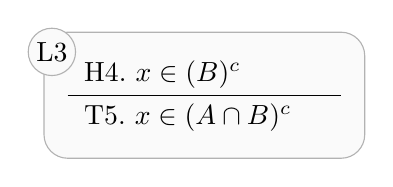
\begin{tikzpicture}[baseline=(main.base)]%
\node[tableau] (main) {%
\\

\begin{tabular}{ll}%
H4.\ $\textrm{$x\in (B)^c$}$&
\Bstrut\\\hline\Tstrut
T5.\ $\textrm{$x\in (A\cap B)^c$}$&
\end{tabular}%
};%
\node[tableaulabel] at (main.north west) [xshift=4mm, yshift=-5.5mm] {L3};
\end{tikzpicture}%

\end{tabular}%
};%
\node[tableaulabel] at (main.north west) [xshift=4mm, yshift=-5.5mm] {L1};
\end{tikzpicture}%
\end{fit}
\smallskip

\noindent6. Quantifier-free expansion of hypothesis H5.\nopagebreak[4] 
\marginpar{Since $x\notin A$, it is not that case that $x\in A$.}\nopagebreak[4] 
\smallskip\nopagebreak[4] 

\begin{fit}\begin{tikzpicture}[baseline=(main.base)]%
\node[tableau] (main) {%
$x$\\

\begin{tabular}{ll}%

\Bstrut\\\hline\Tstrut
\begin{tikzpicture}[baseline=(main.base)]%
\node[tableau] (main) {%
\\

\begin{tabular}{ll}%
H6.\ $\neg \textrm{$x\in A$}$&
\Bstrut\\\hline\Tstrut
T4.\ $\textrm{$x\in (A\cap B)^c$}$&
\end{tabular}%
};%
\node[tableaulabel] at (main.north west) [xshift=4mm, yshift=-5.5mm] {L2};
\end{tikzpicture}%
\\
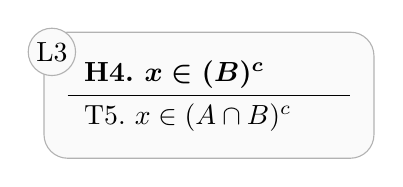
\begin{tikzpicture}[baseline=(main.base)]%
\node[tableau] (main) {%
\\

\begin{tabular}{ll}%
\textbf{\boldmath H4.\ $\textrm{$x\in (B)^c$}$\unboldmath }&\textbf{\boldmath \unboldmath }
\Bstrut\\\hline\Tstrut
T5.\ $\textrm{$x\in (A\cap B)^c$}$&
\end{tabular}%
};%
\node[tableaulabel] at (main.north west) [xshift=4mm, yshift=-5.5mm] {L3};
\end{tikzpicture}%

\end{tabular}%
};%
\node[tableaulabel] at (main.north west) [xshift=4mm, yshift=-5.5mm] {L1};
\end{tikzpicture}%
\end{fit}
\smallskip

\noindent7. Quantifier-free expansion of hypothesis H4.\nopagebreak[4] 
\marginpar{Since $x\in (B)^c$, we have that $x\notin B$.}\nopagebreak[4] 
\smallskip\nopagebreak[4] 

\begin{fit}\begin{tikzpicture}[baseline=(main.base)]%
\node[tableau] (main) {%
$x$\\

\begin{tabular}{ll}%

\Bstrut\\\hline\Tstrut
\begin{tikzpicture}[baseline=(main.base)]%
\node[tableau] (main) {%
\\

\begin{tabular}{ll}%
H6.\ $\neg \textrm{$x\in A$}$&
\Bstrut\\\hline\Tstrut
T4.\ $\textrm{$x\in (A\cap B)^c$}$&
\end{tabular}%
};%
\node[tableaulabel] at (main.north west) [xshift=4mm, yshift=-5.5mm] {L2};
\end{tikzpicture}%
\\
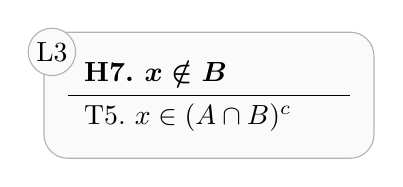
\begin{tikzpicture}[baseline=(main.base)]%
\node[tableau] (main) {%
\\

\begin{tabular}{ll}%
\textbf{\boldmath H7.\ $\textrm{$x\notin B$}$\unboldmath }&\textbf{\boldmath \unboldmath }
\Bstrut\\\hline\Tstrut
T5.\ $\textrm{$x\in (A\cap B)^c$}$&
\end{tabular}%
};%
\node[tableaulabel] at (main.north west) [xshift=4mm, yshift=-5.5mm] {L3};
\end{tikzpicture}%

\end{tabular}%
};%
\node[tableaulabel] at (main.north west) [xshift=4mm, yshift=-5.5mm] {L1};
\end{tikzpicture}%
\end{fit}
\smallskip

\noindent8. Quantifier-free expansion of hypothesis H7.\nopagebreak[4] 
\marginpar{Since $x\notin B$, it is not that case that $x\in B$.}\nopagebreak[4] 
\smallskip\nopagebreak[4] 

\begin{fit}\begin{tikzpicture}[baseline=(main.base)]%
\node[tableau] (main) {%
$x$\\

\begin{tabular}{ll}%

\Bstrut\\\hline\Tstrut
\begin{tikzpicture}[baseline=(main.base)]%
\node[tableau] (main) {%
\\

\begin{tabular}{ll}%
H6.\ $\neg \textrm{$x\in A$}$&
\Bstrut\\\hline\Tstrut
\textbf{\boldmath T4.\ $\textrm{$x\in (A\cap B)^c$}$\unboldmath }&\textbf{\boldmath \unboldmath }
\end{tabular}%
};%
\node[tableaulabel] at (main.north west) [xshift=4mm, yshift=-5.5mm] {L2};
\end{tikzpicture}%
\\
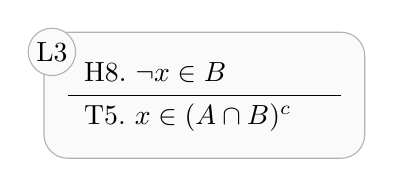
\begin{tikzpicture}[baseline=(main.base)]%
\node[tableau] (main) {%
\\

\begin{tabular}{ll}%
H8.\ $\neg \textrm{$x\in B$}$&
\Bstrut\\\hline\Tstrut
T5.\ $\textrm{$x\in (A\cap B)^c$}$&
\end{tabular}%
};%
\node[tableaulabel] at (main.north west) [xshift=4mm, yshift=-5.5mm] {L3};
\end{tikzpicture}%

\end{tabular}%
};%
\node[tableaulabel] at (main.north west) [xshift=4mm, yshift=-5.5mm] {L1};
\end{tikzpicture}%
\end{fit}
\smallskip

\noindent9. Quantifier-free expansion of target T4.\nopagebreak[4] 
\marginpar{We would like to show that $x\in (A\cap B)^c$, i.e. that $x\notin A\cap B$.}\nopagebreak[4] 
\smallskip\nopagebreak[4] 

\begin{fit}\begin{tikzpicture}[baseline=(main.base)]%
\node[tableau] (main) {%
$x$\\

\begin{tabular}{ll}%

\Bstrut\\\hline\Tstrut
\begin{tikzpicture}[baseline=(main.base)]%
\node[tableau] (main) {%
\\

\begin{tabular}{ll}%
H6.\ $\neg \textrm{$x\in A$}$&
\Bstrut\\\hline\Tstrut
\textbf{\boldmath T6.\ $\textrm{$x\notin A\cap B$}$\unboldmath }&\textbf{\boldmath \unboldmath }
\end{tabular}%
};%
\node[tableaulabel] at (main.north west) [xshift=4mm, yshift=-5.5mm] {L2};
\end{tikzpicture}%
\\
\begin{tikzpicture}[baseline=(main.base)]%
\node[tableau] (main) {%
\\

\begin{tabular}{ll}%
H8.\ $\neg \textrm{$x\in B$}$&
\Bstrut\\\hline\Tstrut
T5.\ $\textrm{$x\in (A\cap B)^c$}$&
\end{tabular}%
};%
\node[tableaulabel] at (main.north west) [xshift=4mm, yshift=-5.5mm] {L3};
\end{tikzpicture}%

\end{tabular}%
};%
\node[tableaulabel] at (main.north west) [xshift=4mm, yshift=-5.5mm] {L1};
\end{tikzpicture}%
\end{fit}
\smallskip

\noindent10. Quantifier-free expansion of target T6.\nopagebreak[4] 
\marginpar{We would like to show that $x\notin A\cap B$, i.e. that it is not that case that $x\in A\cap B$.}\nopagebreak[4] 
\smallskip\nopagebreak[4] 

\begin{fit}\begin{tikzpicture}[baseline=(main.base)]%
\node[tableau] (main) {%
$x$\\

\begin{tabular}{ll}%

\Bstrut\\\hline\Tstrut
\begin{tikzpicture}[baseline=(main.base)]%
\node[tableau] (main) {%
\\

\begin{tabular}{ll}%
H6.\ $\neg \textrm{$x\in A$}$&
\Bstrut\\\hline\Tstrut
T7.\ $\neg \textrm{$x\in A\cap B$}$&
\end{tabular}%
};%
\node[tableaulabel] at (main.north west) [xshift=4mm, yshift=-5.5mm] {L2};
\end{tikzpicture}%
\\
\begin{tikzpicture}[baseline=(main.base)]%
\node[tableau] (main) {%
\\

\begin{tabular}{ll}%
H8.\ $\neg \textrm{$x\in B$}$&
\Bstrut\\\hline\Tstrut
\textbf{\boldmath T5.\ $\textrm{$x\in (A\cap B)^c$}$\unboldmath }&\textbf{\boldmath \unboldmath }
\end{tabular}%
};%
\node[tableaulabel] at (main.north west) [xshift=4mm, yshift=-5.5mm] {L3};
\end{tikzpicture}%

\end{tabular}%
};%
\node[tableaulabel] at (main.north west) [xshift=4mm, yshift=-5.5mm] {L1};
\end{tikzpicture}%
\end{fit}
\smallskip

\noindent11. Quantifier-free expansion of target T5.\nopagebreak[4] 
\marginpar{We would like to show that $x\in (A\cap B)^c$, i.e. that $x\notin A\cap B$.}\nopagebreak[4] 
\smallskip\nopagebreak[4] 

\begin{fit}\begin{tikzpicture}[baseline=(main.base)]%
\node[tableau] (main) {%
$x$\\

\begin{tabular}{ll}%

\Bstrut\\\hline\Tstrut
\begin{tikzpicture}[baseline=(main.base)]%
\node[tableau] (main) {%
\\

\begin{tabular}{ll}%
H6.\ $\neg \textrm{$x\in A$}$&
\Bstrut\\\hline\Tstrut
T7.\ $\neg \textrm{$x\in A\cap B$}$&
\end{tabular}%
};%
\node[tableaulabel] at (main.north west) [xshift=4mm, yshift=-5.5mm] {L2};
\end{tikzpicture}%
\\
\begin{tikzpicture}[baseline=(main.base)]%
\node[tableau] (main) {%
\\

\begin{tabular}{ll}%
H8.\ $\neg \textrm{$x\in B$}$&
\Bstrut\\\hline\Tstrut
\textbf{\boldmath T8.\ $\textrm{$x\notin A\cap B$}$\unboldmath }&\textbf{\boldmath \unboldmath }
\end{tabular}%
};%
\node[tableaulabel] at (main.north west) [xshift=4mm, yshift=-5.5mm] {L3};
\end{tikzpicture}%

\end{tabular}%
};%
\node[tableaulabel] at (main.north west) [xshift=4mm, yshift=-5.5mm] {L1};
\end{tikzpicture}%
\end{fit}
\smallskip

\noindent12. Quantifier-free expansion of target T8.\nopagebreak[4] 
\marginpar{We would like to show that $x\notin A\cap B$, i.e. that it is not that case that $x\in A\cap B$.}\nopagebreak[4] 
\smallskip\nopagebreak[4] 

\begin{fit}\begin{tikzpicture}[baseline=(main.base)]%
\node[tableau] (main) {%
$x$\\

\begin{tabular}{ll}%

\Bstrut\\\hline\Tstrut
\begin{tikzpicture}[baseline=(main.base)]%
\node[tableau] (main) {%
\\

\begin{tabular}{ll}%
H6.\ $\neg \textrm{$x\in A$}$&
\Bstrut\\\hline\Tstrut
T7.\ $\neg \textrm{$x\in A\cap B$}$&
\end{tabular}%
};%
\node[tableaulabel] at (main.north west) [xshift=4mm, yshift=-5.5mm] {L2};
\end{tikzpicture}%
\\
\begin{tikzpicture}[baseline=(main.base)]%
\node[tableau] (main) {%
\\

\begin{tabular}{ll}%
H8.\ $\neg \textrm{$x\in B$}$&
\Bstrut\\\hline\Tstrut
T9.\ $\neg \textrm{$x\in A\cap B$}$&
\end{tabular}%
};%
\node[tableaulabel] at (main.north west) [xshift=4mm, yshift=-5.5mm] {L3};
\end{tikzpicture}%

\end{tabular}%
};%
\node[tableaulabel] at (main.north west) [xshift=4mm, yshift=-5.5mm] {L1};
\end{tikzpicture}%
\end{fit}

No moves possible.
\cleardoublepage

\end{steps}
{\begin{center} \large \textbf{Prove that $(A \cup B)^c = A^c \cap B^c$}\end{center}}\nopagebreak[4]

\begin{center}
\begin{minipage}{120mm}
We would like to show that $(A\cup B)^c\subset (A)^c\cap (B)^c$, i.e. that $(A\cup B)^c\subset (A)^c$ and $(A\cup B)^c\subset (B)^c$.
\end{minipage}
\end{center}

\bigskip
\begin{steps}
\begin{fit}\begin{tikzpicture}[baseline=(main.base)]%
\node[tableau] (main) {%
\\

\begin{tabular}{ll}%

\Bstrut\\\hline\Tstrut
\textbf{\boldmath T1.\ $\textrm{$(A\cup B)^c\subset (A)^c\cap (B)^c$}$\unboldmath }&\textbf{\boldmath \unboldmath }
\end{tabular}%
};%
\node[tableaulabel] at (main.north west) [xshift=4mm, yshift=-5.5mm] {L1};
\end{tikzpicture}%
\end{fit}
\smallskip

\noindent1. Quantifier-free expansion of target T1.\nopagebreak[4] 
\marginpar{We would like to show that $(A\cup B)^c\subset (A)^c\cap (B)^c$, i.e. that $(A\cup B)^c\subset (A)^c$ and $(A\cup B)^c\subset (B)^c$.}\nopagebreak[4] 
\smallskip\nopagebreak[4] 

\begin{fit}\begin{tikzpicture}[baseline=(main.base)]%
\node[tableau] (main) {%
\\

\begin{tabular}{ll}%

\Bstrut\\\hline\Tstrut
T2.\ $\textrm{$(A\cup B)^c\subset (A)^c$}$&\\
T3.\ $\textrm{$(A\cup B)^c\subset (B)^c$}$&
\end{tabular}%
};%
\node[tableaulabel] at (main.north west) [xshift=4mm, yshift=-5.5mm] {L1};
\end{tikzpicture}%
\end{fit}

No moves possible.
\cleardoublepage

\end{steps}
{\begin{center} \large \textbf{Prove that $A^c \cap B^c \subseteq (A \cup B)^c$.}\end{center}}\nopagebreak[4]

\begin{center}
\begin{minipage}{120mm}
Let $x$ be an element of $(A)^c\cap (B)^c$. Then $x\in (A)^c$ and $x\in (B)^c$. Then $x\notin A\cup B$ and $x\notin A$. Then it is not that case that $x\in A$. Since $x\in (B)^c$, we have that $x\notin B$. Then it is not that case that $x\in B$. Since $x\notin A\cup B$, it is not that case that $x\in A\cup B$. We would like to show that $x\in (A\cup B)^c$, i.e. that $x\notin A\cup B$. We would like to show that $x\notin A\cup B$, i.e. that it is not that case that $x\in A\cup B$. But this is clearly the case, so we are done.
\end{minipage}
\end{center}

\bigskip
\begin{steps}
\begin{fit}\begin{tikzpicture}[baseline=(main.base)]%
\node[tableau] (main) {%
\\

\begin{tabular}{ll}%

\Bstrut\\\hline\Tstrut
\textbf{\boldmath T1.\ $\textrm{$(A)^c\cap (B)^c\subset (A\cup B)^c$}$\unboldmath }&\textbf{\boldmath \unboldmath }
\end{tabular}%
};%
\node[tableaulabel] at (main.north west) [xshift=4mm, yshift=-5.5mm] {L1};
\end{tikzpicture}%
\end{fit}
\smallskip

\noindent1. Expand pre-universal target T1.\nopagebreak[4] 
\marginpar{}\nopagebreak[4] 
\smallskip\nopagebreak[4] 

\begin{fit}\begin{tikzpicture}[baseline=(main.base)]%
\node[tableau] (main) {%
\\

\begin{tabular}{ll}%

\Bstrut\\\hline\Tstrut
\textbf{\boldmath T2.\ $\forall x.(\textrm{$x\in (A)^c\cap (B)^c$}\Rightarrow \textrm{$x\in (A\cup B)^c$})$\unboldmath }&\textbf{\boldmath \unboldmath }
\end{tabular}%
};%
\node[tableaulabel] at (main.north west) [xshift=4mm, yshift=-5.5mm] {L1};
\end{tikzpicture}%
\end{fit}
\smallskip

\noindent2. Apply `let' trick and move premise of universal-conditional target T2 above the line.\nopagebreak[4] 
\marginpar{Let $x$ be an element of $(A)^c\cap (B)^c$.}\nopagebreak[4] 
\smallskip\nopagebreak[4] 

\begin{fit}\begin{tikzpicture}[baseline=(main.base)]%
\node[tableau] (main) {%
$x$\\

\begin{tabular}{ll}%
\textbf{\boldmath H1.\ $\textrm{$x\in (A)^c\cap (B)^c$}$\unboldmath }&\textbf{\boldmath \unboldmath }
\Bstrut\\\hline\Tstrut
T3.\ $\textrm{$x\in (A\cup B)^c$}$&
\end{tabular}%
};%
\node[tableaulabel] at (main.north west) [xshift=4mm, yshift=-5.5mm] {L1};
\end{tikzpicture}%
\end{fit}
\smallskip

\noindent3. Quantifier-free expansion of hypothesis H1.\nopagebreak[4] 
\marginpar{Since $x\in (A)^c\cap (B)^c$, $x\in (A)^c$ and $x\in (B)^c$.}\nopagebreak[4] 
\smallskip\nopagebreak[4] 

\begin{fit}\begin{tikzpicture}[baseline=(main.base)]%
\node[tableau] (main) {%
$x$\\

\begin{tabular}{ll}%
\textbf{\boldmath H2.\ $\textrm{$x\in (A)^c$}$\unboldmath }&\textbf{\boldmath \unboldmath }\\
\textbf{\boldmath H3.\ $\textrm{$x\in (B)^c$}$\unboldmath }&\textbf{\boldmath \unboldmath }
\Bstrut\\\hline\Tstrut
T3.\ $\textrm{$x\in (A\cup B)^c$}$&
\end{tabular}%
};%
\node[tableaulabel] at (main.north west) [xshift=4mm, yshift=-5.5mm] {L1};
\end{tikzpicture}%
\end{fit}
\smallskip

\noindent4. Forwards reasoning using library result ``'' with (H2,H3).\nopagebreak[4] 
\marginpar{Since $x\in (A)^c$ and $x\in (B)^c$, we have that $x\notin A\cup B$.}\nopagebreak[4] 
\smallskip\nopagebreak[4] 

\begin{fit}\begin{tikzpicture}[baseline=(main.base)]%
\node[tableau] (main) {%
$x$\\

\begin{tabular}{ll}%
\textbf{\boldmath H2.\ $\textrm{$x\in (A)^c$}$\unboldmath }&\textbf{\boldmath [Vuln.]\unboldmath }\\
H3.\ $\textrm{$x\in (B)^c$}$&[Vuln.]\\
H4.\ $\textrm{$x\notin A\cup B$}$&
\Bstrut\\\hline\Tstrut
T3.\ $\textrm{$x\in (A\cup B)^c$}$&
\end{tabular}%
};%
\node[tableaulabel] at (main.north west) [xshift=4mm, yshift=-5.5mm] {L1};
\end{tikzpicture}%
\end{fit}
\smallskip

\noindent5. Quantifier-free expansion of hypothesis H2.\nopagebreak[4] 
\marginpar{Since $x\in (A)^c$, we have that $x\notin A$.}\nopagebreak[4] 
\smallskip\nopagebreak[4] 

\begin{fit}\begin{tikzpicture}[baseline=(main.base)]%
\node[tableau] (main) {%
$x$\\

\begin{tabular}{ll}%
\textbf{\boldmath H5.\ $\textrm{$x\notin A$}$\unboldmath }&\textbf{\boldmath \unboldmath }\\
H3.\ $\textrm{$x\in (B)^c$}$&[Vuln.]\\
H4.\ $\textrm{$x\notin A\cup B$}$&
\Bstrut\\\hline\Tstrut
T3.\ $\textrm{$x\in (A\cup B)^c$}$&
\end{tabular}%
};%
\node[tableaulabel] at (main.north west) [xshift=4mm, yshift=-5.5mm] {L1};
\end{tikzpicture}%
\end{fit}
\smallskip

\noindent6. Quantifier-free expansion of hypothesis H5.\nopagebreak[4] 
\marginpar{Since $x\notin A$, it is not that case that $x\in A$.}\nopagebreak[4] 
\smallskip\nopagebreak[4] 

\begin{fit}\begin{tikzpicture}[baseline=(main.base)]%
\node[tableau] (main) {%
$x$\\

\begin{tabular}{ll}%
H6.\ $\neg \textrm{$x\in A$}$&\\
\textbf{\boldmath H3.\ $\textrm{$x\in (B)^c$}$\unboldmath }&\textbf{\boldmath [Vuln.]\unboldmath }\\
H4.\ $\textrm{$x\notin A\cup B$}$&
\Bstrut\\\hline\Tstrut
T3.\ $\textrm{$x\in (A\cup B)^c$}$&
\end{tabular}%
};%
\node[tableaulabel] at (main.north west) [xshift=4mm, yshift=-5.5mm] {L1};
\end{tikzpicture}%
\end{fit}
\smallskip

\noindent7. Quantifier-free expansion of hypothesis H3.\nopagebreak[4] 
\marginpar{Since $x\in (B)^c$, we have that $x\notin B$.}\nopagebreak[4] 
\smallskip\nopagebreak[4] 

\begin{fit}\begin{tikzpicture}[baseline=(main.base)]%
\node[tableau] (main) {%
$x$\\

\begin{tabular}{ll}%
H6.\ $\neg \textrm{$x\in A$}$&\\
\textbf{\boldmath H7.\ $\textrm{$x\notin B$}$\unboldmath }&\textbf{\boldmath \unboldmath }\\
H4.\ $\textrm{$x\notin A\cup B$}$&
\Bstrut\\\hline\Tstrut
T3.\ $\textrm{$x\in (A\cup B)^c$}$&
\end{tabular}%
};%
\node[tableaulabel] at (main.north west) [xshift=4mm, yshift=-5.5mm] {L1};
\end{tikzpicture}%
\end{fit}
\smallskip

\noindent8. Quantifier-free expansion of hypothesis H7.\nopagebreak[4] 
\marginpar{Since $x\notin B$, it is not that case that $x\in B$.}\nopagebreak[4] 
\smallskip\nopagebreak[4] 

\begin{fit}\begin{tikzpicture}[baseline=(main.base)]%
\node[tableau] (main) {%
$x$\\

\begin{tabular}{ll}%
H6.\ $\neg \textrm{$x\in A$}$&\\
H8.\ $\neg \textrm{$x\in B$}$&\\
\textbf{\boldmath H4.\ $\textrm{$x\notin A\cup B$}$\unboldmath }&\textbf{\boldmath \unboldmath }
\Bstrut\\\hline\Tstrut
T3.\ $\textrm{$x\in (A\cup B)^c$}$&
\end{tabular}%
};%
\node[tableaulabel] at (main.north west) [xshift=4mm, yshift=-5.5mm] {L1};
\end{tikzpicture}%
\end{fit}
\smallskip

\noindent9. Quantifier-free expansion of hypothesis H4.\nopagebreak[4] 
\marginpar{Since $x\notin A\cup B$, it is not that case that $x\in A\cup B$.}\nopagebreak[4] 
\smallskip\nopagebreak[4] 

\begin{fit}\begin{tikzpicture}[baseline=(main.base)]%
\node[tableau] (main) {%
$x$\\

\begin{tabular}{ll}%
H6.\ $\neg \textrm{$x\in A$}$&\\
H8.\ $\neg \textrm{$x\in B$}$&\\
H9.\ $\neg \textrm{$x\in A\cup B$}$&
\Bstrut\\\hline\Tstrut
\textbf{\boldmath T3.\ $\textrm{$x\in (A\cup B)^c$}$\unboldmath }&\textbf{\boldmath \unboldmath }
\end{tabular}%
};%
\node[tableaulabel] at (main.north west) [xshift=4mm, yshift=-5.5mm] {L1};
\end{tikzpicture}%
\end{fit}
\smallskip

\noindent10. Quantifier-free expansion of target T3.\nopagebreak[4] 
\marginpar{We would like to show that $x\in (A\cup B)^c$, i.e. that $x\notin A\cup B$.}\nopagebreak[4] 
\smallskip\nopagebreak[4] 

\begin{fit}\begin{tikzpicture}[baseline=(main.base)]%
\node[tableau] (main) {%
$x$\\

\begin{tabular}{ll}%
H6.\ $\neg \textrm{$x\in A$}$&\\
H8.\ $\neg \textrm{$x\in B$}$&\\
H9.\ $\neg \textrm{$x\in A\cup B$}$&
\Bstrut\\\hline\Tstrut
\textbf{\boldmath T4.\ $\textrm{$x\notin A\cup B$}$\unboldmath }&\textbf{\boldmath \unboldmath }
\end{tabular}%
};%
\node[tableaulabel] at (main.north west) [xshift=4mm, yshift=-5.5mm] {L1};
\end{tikzpicture}%
\end{fit}
\smallskip

\noindent11. Quantifier-free expansion of target T4.\nopagebreak[4] 
\marginpar{We would like to show that $x\notin A\cup B$, i.e. that it is not that case that $x\in A\cup B$.}\nopagebreak[4] 
\smallskip\nopagebreak[4] 

\begin{fit}\begin{tikzpicture}[baseline=(main.base)]%
\node[tableau] (main) {%
$x$\\

\begin{tabular}{ll}%
H6.\ $\neg \textrm{$x\in A$}$&\\
H8.\ $\neg \textrm{$x\in B$}$&\\
\textbf{\boldmath H9.\ $\neg \textrm{$x\in A\cup B$}$\unboldmath }&\textbf{\boldmath \unboldmath }
\Bstrut\\\hline\Tstrut
\textbf{\boldmath T5.\ $\neg \textrm{$x\in A\cup B$}$\unboldmath }&\textbf{\boldmath \unboldmath }
\end{tabular}%
};%
\node[tableaulabel] at (main.north west) [xshift=4mm, yshift=-5.5mm] {L1};
\end{tikzpicture}%
\end{fit}
\smallskip

\noindent12. Hypothesis H9 matches target T5, so L1 is done.\nopagebreak[4] 
\marginpar{But this is clearly the case, so we are done.}\nopagebreak[4] 
\smallskip\nopagebreak[4] 

\begin{fit}\begin{tikzpicture}%
\node[tableau] (main) {%
\ \ \,Done
};%
\node[tableaulabel] at (main.north west) [xshift=4mm, yshift=-5.5mm] {L1};
\end{tikzpicture}%
\end{fit}

Problem solved.
\cleardoublepage

\end{steps}
{\begin{center} \large \textbf{If $A$, $B$,and $C$ are open sets, then $A \cap (B \cap C)$ is also open.}\end{center}}\nopagebreak[4]

\begin{center}
\begin{minipage}{120mm}
Let $x$ be an element of $A\cap B\cap C$. Then $x\in A$ and $x\in B\cap C$. Therefore, since $A$ is open, there exists $\eta > 0$ such that $u\in A$\textrm{ whenever }$\textit{d}(x,u) < \eta$ and $x\in B$ and $x\in C$. Therefore, since $B$ is open, there exists $\theta > 0$ such that $v\in B$\textrm{ whenever }$\textit{d}(x,v) < \theta$ and since $C$ is open, there exists $\alpha > 0$ such that $w\in C$\textrm{ whenever }$\textit{d}(x,w) < \alpha$. We would like to find $\delta > 0$ s.t. $y\in A\cap B\cap C$\textrm{ whenever }$\textit{d}(x,y) < \delta$. But $y\in A\cap B\cap C$ if and only if $y\in A$ and $y\in B\cap C$. We know that $y\in A$ whenever $\textit{d}(x,y) < \eta$. But $y\in B\cap C$ if and only if $y\in B$ and $y\in C$. We know that $y\in B$ whenever $\textit{d}(x,y) < \theta$ and that $y\in C$ whenever $\textit{d}(x,y) < \alpha$. Assume now that $\textit{d}(x,y) < \delta$. Then $\textit{d}(x,y) < \eta$ if $\delta\leqslant \eta$, $\textit{d}(x,y) < \theta$ if $\delta\leqslant \theta$ and $\textit{d}(x,y) < \alpha$ if $\delta\leqslant \alpha$.
\end{minipage}
\end{center}

\bigskip
\begin{steps}
\begin{fit}\begin{tikzpicture}[baseline=(main.base)]%
\node[tableau] (main) {%
\\

\begin{tabular}{ll}%
H1.\ $\textrm{$A$ is open}$&\\
H2.\ $\textrm{$B$ is open}$&\\
H3.\ $\textrm{$C$ is open}$&
\Bstrut\\\hline\Tstrut
\textbf{\boldmath T1.\ $\textrm{$A\cap B\cap C$ is open}$\unboldmath }&\textbf{\boldmath \unboldmath }
\end{tabular}%
};%
\node[tableaulabel] at (main.north west) [xshift=4mm, yshift=-5.5mm] {L1};
\end{tikzpicture}%
\end{fit}
\smallskip

\noindent1. Expand pre-universal target T1.\nopagebreak[4] 
\marginpar{}\nopagebreak[4] 
\smallskip\nopagebreak[4] 

\begin{fit}\begin{tikzpicture}[baseline=(main.base)]%
\node[tableau] (main) {%
\\

\begin{tabular}{ll}%
H1.\ $\textrm{$A$ is open}$&\\
H2.\ $\textrm{$B$ is open}$&\\
H3.\ $\textrm{$C$ is open}$&
\Bstrut\\\hline\Tstrut
\textbf{\boldmath T2.\ $\forall x.(\textrm{$x\in A\cap B\cap C$}\Rightarrow \exists \delta.(\forall y.(\textrm{$\textit{d}(x,y) < \delta$}\Rightarrow \textrm{$y\in A\cap B\cap C$})))$\unboldmath }&\textbf{\boldmath \unboldmath }
\end{tabular}%
};%
\node[tableaulabel] at (main.north west) [xshift=4mm, yshift=-5.5mm] {L1};
\end{tikzpicture}%
\end{fit}
\smallskip

\noindent2. Apply `let' trick and move premise of universal-conditional target T2 above the line.\nopagebreak[4] 
\marginpar{Let $x$ be an element of $A\cap B\cap C$.}\nopagebreak[4] 
\smallskip\nopagebreak[4] 

\begin{fit}\begin{tikzpicture}[baseline=(main.base)]%
\node[tableau] (main) {%
$x$\\

\begin{tabular}{ll}%
H1.\ $\textrm{$A$ is open}$&\\
H2.\ $\textrm{$B$ is open}$&\\
H3.\ $\textrm{$C$ is open}$&\\
\textbf{\boldmath H4.\ $\textrm{$x\in A\cap B\cap C$}$\unboldmath }&\textbf{\boldmath \unboldmath }
\Bstrut\\\hline\Tstrut
T3.\ $\exists \delta.(\forall y.(\textrm{$\textit{d}(x,y) < \delta$}\Rightarrow \textrm{$y\in A\cap B\cap C$}))$&
\end{tabular}%
};%
\node[tableaulabel] at (main.north west) [xshift=4mm, yshift=-5.5mm] {L1};
\end{tikzpicture}%
\end{fit}
\smallskip

\noindent3. Quantifier-free expansion of hypothesis H4.\nopagebreak[4] 
\marginpar{Since $x\in A\cap B\cap C$, $x\in A$ and $x\in B\cap C$.}\nopagebreak[4] 
\smallskip\nopagebreak[4] 

\begin{fit}\begin{tikzpicture}[baseline=(main.base)]%
\node[tableau] (main) {%
$x$\\

\begin{tabular}{ll}%
\textbf{\boldmath H1.\ $\textrm{$A$ is open}$\unboldmath }&\textbf{\boldmath \unboldmath }\\
H2.\ $\textrm{$B$ is open}$&\\
H3.\ $\textrm{$C$ is open}$&\\
\textbf{\boldmath H5.\ $\textrm{$x\in A$}$\unboldmath }&\textbf{\boldmath \unboldmath }\\
H6.\ $\textrm{$x\in B\cap C$}$&
\Bstrut\\\hline\Tstrut
T3.\ $\exists \delta.(\forall y.(\textrm{$\textit{d}(x,y) < \delta$}\Rightarrow \textrm{$y\in A\cap B\cap C$}))$&
\end{tabular}%
};%
\node[tableaulabel] at (main.north west) [xshift=4mm, yshift=-5.5mm] {L1};
\end{tikzpicture}%
\end{fit}
\smallskip

\noindent4. Forwards reasoning using H1 with H5.\nopagebreak[4] 
\marginpar{Since $A$ is open and $x\in A$, there exists $\eta > 0$ such that $u\in A$\textrm{ whenever }$\textit{d}(x,u) < \eta$.}\nopagebreak[4] 
\smallskip\nopagebreak[4] 

\begin{fit}\begin{tikzpicture}[baseline=(main.base)]%
\node[tableau] (main) {%
$x$\hspace{1.5mm}$\eta[x]$\\

\begin{tabular}{ll}%
H1.\ $\textrm{$A$ is open}$&[Vuln.; Used with H5.]\\
H2.\ $\textrm{$B$ is open}$&\\
H3.\ $\textrm{$C$ is open}$&\\
H5.\ $\textrm{$x\in A$}$&[Vuln.]\\
H6.\ $\textrm{$x\in B\cap C$}$&\\
H7.\ $\forall u.(\textrm{$\textit{d}(x,u) < \eta[x]$}\Rightarrow \textrm{$u\in A$})$&
\Bstrut\\\hline\Tstrut
T3.\ $\exists \delta.(\forall y.(\textrm{$\textit{d}(x,y) < \delta$}\Rightarrow \textrm{$y\in A\cap B\cap C$}))$&
\end{tabular}%
};%
\node[tableaulabel] at (main.north west) [xshift=4mm, yshift=-5.5mm] {L1};
\end{tikzpicture}%
\end{fit}
\smallskip

\noindent5. Deleted H5, as this unexpandable atomic statement is unmatchable.\nopagebreak[4] 
\marginpar{}\nopagebreak[4] 
\smallskip\nopagebreak[4] 

\begin{fit}\begin{tikzpicture}[baseline=(main.base)]%
\node[tableau] (main) {%
$x$\hspace{1.5mm}$\eta[x]$\\

\begin{tabular}{ll}%
H1.\ $\textrm{$A$ is open}$&[Vuln.; Used with H5.]\\
H2.\ $\textrm{$B$ is open}$&\\
H3.\ $\textrm{$C$ is open}$&\\
\grey{H5.\ $\textrm{$x\in A$}$}&\grey{[Vuln.]}\\
H6.\ $\textrm{$x\in B\cap C$}$&\\
H7.\ $\forall u.(\textrm{$\textit{d}(x,u) < \eta[x]$}\Rightarrow \textrm{$u\in A$})$&
\Bstrut\\\hline\Tstrut
T3.\ $\exists \delta.(\forall y.(\textrm{$\textit{d}(x,y) < \delta$}\Rightarrow \textrm{$y\in A\cap B\cap C$}))$&
\end{tabular}%
};%
\node[tableaulabel] at (main.north west) [xshift=4mm, yshift=-5.5mm] {L1};
\end{tikzpicture}%
\end{fit}
\smallskip

\noindent6. Deleted H1, as the conclusion of this implicative statement is unmatchable.\nopagebreak[4] 
\marginpar{}\nopagebreak[4] 
\smallskip\nopagebreak[4] 

\begin{fit}\begin{tikzpicture}[baseline=(main.base)]%
\node[tableau] (main) {%
$x$\hspace{1.5mm}$\eta[x]$\\

\begin{tabular}{ll}%
\grey{H1.\ $\textrm{$A$ is open}$}&\grey{[Vuln.; Used with H5.]}\\
H2.\ $\textrm{$B$ is open}$&\\
H3.\ $\textrm{$C$ is open}$&\\
\grey{H5.\ $\textrm{$x\in A$}$}&\grey{[Vuln.]}\\
\textbf{\boldmath H6.\ $\textrm{$x\in B\cap C$}$\unboldmath }&\textbf{\boldmath \unboldmath }\\
H7.\ $\forall u.(\textrm{$\textit{d}(x,u) < \eta[x]$}\Rightarrow \textrm{$u\in A$})$&
\Bstrut\\\hline\Tstrut
T3.\ $\exists \delta.(\forall y.(\textrm{$\textit{d}(x,y) < \delta$}\Rightarrow \textrm{$y\in A\cap B\cap C$}))$&
\end{tabular}%
};%
\node[tableaulabel] at (main.north west) [xshift=4mm, yshift=-5.5mm] {L1};
\end{tikzpicture}%
\end{fit}
\smallskip

\noindent7. Quantifier-free expansion of hypothesis H6.\nopagebreak[4] 
\marginpar{Since $x\in B\cap C$, $x\in B$ and $x\in C$.}\nopagebreak[4] 
\smallskip\nopagebreak[4] 

\begin{fit}\begin{tikzpicture}[baseline=(main.base)]%
\node[tableau] (main) {%
$x$\hspace{1.5mm}$\eta[x]$\\

\begin{tabular}{ll}%
\grey{H1.\ $\textrm{$A$ is open}$}&\grey{[Vuln.; Used with H5.]}\\
\textbf{\boldmath H2.\ $\textrm{$B$ is open}$\unboldmath }&\textbf{\boldmath \unboldmath }\\
H3.\ $\textrm{$C$ is open}$&\\
\grey{H5.\ $\textrm{$x\in A$}$}&\grey{[Vuln.]}\\
\textbf{\boldmath H8.\ $\textrm{$x\in B$}$\unboldmath }&\textbf{\boldmath \unboldmath }\\
H9.\ $\textrm{$x\in C$}$&\\
H7.\ $\forall u.(\textrm{$\textit{d}(x,u) < \eta[x]$}\Rightarrow \textrm{$u\in A$})$&
\Bstrut\\\hline\Tstrut
T3.\ $\exists \delta.(\forall y.(\textrm{$\textit{d}(x,y) < \delta$}\Rightarrow \textrm{$y\in A\cap B\cap C$}))$&
\end{tabular}%
};%
\node[tableaulabel] at (main.north west) [xshift=4mm, yshift=-5.5mm] {L1};
\end{tikzpicture}%
\end{fit}
\smallskip

\noindent8. Forwards reasoning using H2 with H8.\nopagebreak[4] 
\marginpar{Since $B$ is open and $x\in B$, there exists $\theta > 0$ such that $v\in B$\textrm{ whenever }$\textit{d}(x,v) < \theta$.}\nopagebreak[4] 
\smallskip\nopagebreak[4] 

\begin{fit}\begin{tikzpicture}[baseline=(main.base)]%
\node[tableau] (main) {%
$x$\hspace{1.5mm}$\eta[x]$\hspace{1.5mm}$\theta[x]$\\

\begin{tabular}{ll}%
\grey{H1.\ $\textrm{$A$ is open}$}&\grey{[Vuln.; Used with H5.]}\\
H2.\ $\textrm{$B$ is open}$&[Vuln.; Used with H8.]\\
H3.\ $\textrm{$C$ is open}$&\\
\grey{H5.\ $\textrm{$x\in A$}$}&\grey{[Vuln.]}\\
H8.\ $\textrm{$x\in B$}$&[Vuln.]\\
H9.\ $\textrm{$x\in C$}$&\\
H7.\ $\forall u.(\textrm{$\textit{d}(x,u) < \eta[x]$}\Rightarrow \textrm{$u\in A$})$&\\
H10.\ $\forall v.(\textrm{$\textit{d}(x,v) < \theta[x]$}\Rightarrow \textrm{$v\in B$})$&
\Bstrut\\\hline\Tstrut
T3.\ $\exists \delta.(\forall y.(\textrm{$\textit{d}(x,y) < \delta$}\Rightarrow \textrm{$y\in A\cap B\cap C$}))$&
\end{tabular}%
};%
\node[tableaulabel] at (main.north west) [xshift=4mm, yshift=-5.5mm] {L1};
\end{tikzpicture}%
\end{fit}
\smallskip

\noindent9. Deleted H8, as this unexpandable atomic statement is unmatchable.\nopagebreak[4] 
\marginpar{}\nopagebreak[4] 
\smallskip\nopagebreak[4] 

\begin{fit}\begin{tikzpicture}[baseline=(main.base)]%
\node[tableau] (main) {%
$x$\hspace{1.5mm}$\eta[x]$\hspace{1.5mm}$\theta[x]$\\

\begin{tabular}{ll}%
\grey{H1.\ $\textrm{$A$ is open}$}&\grey{[Vuln.; Used with H5.]}\\
H2.\ $\textrm{$B$ is open}$&[Vuln.; Used with H8.]\\
H3.\ $\textrm{$C$ is open}$&\\
\grey{H5.\ $\textrm{$x\in A$}$}&\grey{[Vuln.]}\\
\grey{H8.\ $\textrm{$x\in B$}$}&\grey{[Vuln.]}\\
H9.\ $\textrm{$x\in C$}$&\\
H7.\ $\forall u.(\textrm{$\textit{d}(x,u) < \eta[x]$}\Rightarrow \textrm{$u\in A$})$&\\
H10.\ $\forall v.(\textrm{$\textit{d}(x,v) < \theta[x]$}\Rightarrow \textrm{$v\in B$})$&
\Bstrut\\\hline\Tstrut
T3.\ $\exists \delta.(\forall y.(\textrm{$\textit{d}(x,y) < \delta$}\Rightarrow \textrm{$y\in A\cap B\cap C$}))$&
\end{tabular}%
};%
\node[tableaulabel] at (main.north west) [xshift=4mm, yshift=-5.5mm] {L1};
\end{tikzpicture}%
\end{fit}
\smallskip

\noindent10. Deleted H2, as the conclusion of this implicative statement is unmatchable.\nopagebreak[4] 
\marginpar{}\nopagebreak[4] 
\smallskip\nopagebreak[4] 

\begin{fit}\begin{tikzpicture}[baseline=(main.base)]%
\node[tableau] (main) {%
$x$\hspace{1.5mm}$\eta[x]$\hspace{1.5mm}$\theta[x]$\\

\begin{tabular}{ll}%
\grey{H1.\ $\textrm{$A$ is open}$}&\grey{[Vuln.; Used with H5.]}\\
\grey{H2.\ $\textrm{$B$ is open}$}&\grey{[Vuln.; Used with H8.]}\\
\textbf{\boldmath H3.\ $\textrm{$C$ is open}$\unboldmath }&\textbf{\boldmath \unboldmath }\\
\grey{H5.\ $\textrm{$x\in A$}$}&\grey{[Vuln.]}\\
\grey{H8.\ $\textrm{$x\in B$}$}&\grey{[Vuln.]}\\
\textbf{\boldmath H9.\ $\textrm{$x\in C$}$\unboldmath }&\textbf{\boldmath \unboldmath }\\
H7.\ $\forall u.(\textrm{$\textit{d}(x,u) < \eta[x]$}\Rightarrow \textrm{$u\in A$})$&\\
H10.\ $\forall v.(\textrm{$\textit{d}(x,v) < \theta[x]$}\Rightarrow \textrm{$v\in B$})$&
\Bstrut\\\hline\Tstrut
T3.\ $\exists \delta.(\forall y.(\textrm{$\textit{d}(x,y) < \delta$}\Rightarrow \textrm{$y\in A\cap B\cap C$}))$&
\end{tabular}%
};%
\node[tableaulabel] at (main.north west) [xshift=4mm, yshift=-5.5mm] {L1};
\end{tikzpicture}%
\end{fit}
\smallskip

\noindent11. Forwards reasoning using H3 with H9.\nopagebreak[4] 
\marginpar{Since $C$ is open and $x\in C$, there exists $\alpha > 0$ such that $w\in C$\textrm{ whenever }$\textit{d}(x,w) < \alpha$.}\nopagebreak[4] 
\smallskip\nopagebreak[4] 

\begin{fit}\begin{tikzpicture}[baseline=(main.base)]%
\node[tableau] (main) {%
$x$\hspace{1.5mm}$\eta[x]$\hspace{1.5mm}$\theta[x]$\hspace{1.5mm}$\alpha[x]$\\

\begin{tabular}{ll}%
\grey{H1.\ $\textrm{$A$ is open}$}&\grey{[Vuln.; Used with H5.]}\\
\grey{H2.\ $\textrm{$B$ is open}$}&\grey{[Vuln.; Used with H8.]}\\
H3.\ $\textrm{$C$ is open}$&[Vuln.; Used with H9.]\\
\grey{H5.\ $\textrm{$x\in A$}$}&\grey{[Vuln.]}\\
\grey{H8.\ $\textrm{$x\in B$}$}&\grey{[Vuln.]}\\
H9.\ $\textrm{$x\in C$}$&[Vuln.]\\
H7.\ $\forall u.(\textrm{$\textit{d}(x,u) < \eta[x]$}\Rightarrow \textrm{$u\in A$})$&\\
H10.\ $\forall v.(\textrm{$\textit{d}(x,v) < \theta[x]$}\Rightarrow \textrm{$v\in B$})$&\\
H11.\ $\forall w.(\textrm{$\textit{d}(x,w) < \alpha[x]$}\Rightarrow \textrm{$w\in C$})$&
\Bstrut\\\hline\Tstrut
T3.\ $\exists \delta.(\forall y.(\textrm{$\textit{d}(x,y) < \delta$}\Rightarrow \textrm{$y\in A\cap B\cap C$}))$&
\end{tabular}%
};%
\node[tableaulabel] at (main.north west) [xshift=4mm, yshift=-5.5mm] {L1};
\end{tikzpicture}%
\end{fit}
\smallskip

\noindent12. Deleted H9, as this unexpandable atomic statement is unmatchable.\nopagebreak[4] 
\marginpar{}\nopagebreak[4] 
\smallskip\nopagebreak[4] 

\begin{fit}\begin{tikzpicture}[baseline=(main.base)]%
\node[tableau] (main) {%
$x$\hspace{1.5mm}$\eta[x]$\hspace{1.5mm}$\theta[x]$\hspace{1.5mm}$\alpha[x]$\\

\begin{tabular}{ll}%
\grey{H1.\ $\textrm{$A$ is open}$}&\grey{[Vuln.; Used with H5.]}\\
\grey{H2.\ $\textrm{$B$ is open}$}&\grey{[Vuln.; Used with H8.]}\\
H3.\ $\textrm{$C$ is open}$&[Vuln.; Used with H9.]\\
\grey{H5.\ $\textrm{$x\in A$}$}&\grey{[Vuln.]}\\
\grey{H8.\ $\textrm{$x\in B$}$}&\grey{[Vuln.]}\\
\grey{H9.\ $\textrm{$x\in C$}$}&\grey{[Vuln.]}\\
H7.\ $\forall u.(\textrm{$\textit{d}(x,u) < \eta[x]$}\Rightarrow \textrm{$u\in A$})$&\\
H10.\ $\forall v.(\textrm{$\textit{d}(x,v) < \theta[x]$}\Rightarrow \textrm{$v\in B$})$&\\
H11.\ $\forall w.(\textrm{$\textit{d}(x,w) < \alpha[x]$}\Rightarrow \textrm{$w\in C$})$&
\Bstrut\\\hline\Tstrut
T3.\ $\exists \delta.(\forall y.(\textrm{$\textit{d}(x,y) < \delta$}\Rightarrow \textrm{$y\in A\cap B\cap C$}))$&
\end{tabular}%
};%
\node[tableaulabel] at (main.north west) [xshift=4mm, yshift=-5.5mm] {L1};
\end{tikzpicture}%
\end{fit}
\smallskip

\noindent13. Deleted H3, as the conclusion of this implicative statement is unmatchable.\nopagebreak[4] 
\marginpar{}\nopagebreak[4] 
\smallskip\nopagebreak[4] 

\begin{fit}\begin{tikzpicture}[baseline=(main.base)]%
\node[tableau] (main) {%
$x$\hspace{1.5mm}$\eta[x]$\hspace{1.5mm}$\theta[x]$\hspace{1.5mm}$\alpha[x]$\\

\begin{tabular}{ll}%
\grey{H1.\ $\textrm{$A$ is open}$}&\grey{[Vuln.; Used with H5.]}\\
\grey{H2.\ $\textrm{$B$ is open}$}&\grey{[Vuln.; Used with H8.]}\\
\grey{H3.\ $\textrm{$C$ is open}$}&\grey{[Vuln.; Used with H9.]}\\
\grey{H5.\ $\textrm{$x\in A$}$}&\grey{[Vuln.]}\\
\grey{H8.\ $\textrm{$x\in B$}$}&\grey{[Vuln.]}\\
\grey{H9.\ $\textrm{$x\in C$}$}&\grey{[Vuln.]}\\
H7.\ $\forall u.(\textrm{$\textit{d}(x,u) < \eta[x]$}\Rightarrow \textrm{$u\in A$})$&\\
H10.\ $\forall v.(\textrm{$\textit{d}(x,v) < \theta[x]$}\Rightarrow \textrm{$v\in B$})$&\\
H11.\ $\forall w.(\textrm{$\textit{d}(x,w) < \alpha[x]$}\Rightarrow \textrm{$w\in C$})$&
\Bstrut\\\hline\Tstrut
\textbf{\boldmath T3.\ $\exists \delta.(\forall y.(\textrm{$\textit{d}(x,y) < \delta$}\Rightarrow \textrm{$y\in A\cap B\cap C$}))$\unboldmath }&\textbf{\boldmath \unboldmath }
\end{tabular}%
};%
\node[tableaulabel] at (main.north west) [xshift=4mm, yshift=-5.5mm] {L1};
\end{tikzpicture}%
\end{fit}
\smallskip

\noindent14. Unlock existential-universal-conditional target T3.\nopagebreak[4] 
\marginpar{We would like to find $\delta > 0$ s.t. $y\in A\cap B\cap C$\textrm{ whenever }$\textit{d}(x,y) < \delta$.}\nopagebreak[4] 
\smallskip\nopagebreak[4] 

\begin{fit}\begin{tikzpicture}[baseline=(main.base)]%
\node[tableau] (main) {%
$x$\hspace{1.5mm}$\eta[x]$\hspace{1.5mm}$\theta[x]$\hspace{1.5mm}$\alpha[x]$\\

\begin{tabular}{ll}%
\grey{H1.\ $\textrm{$A$ is open}$}&\grey{[Vuln.; Used with H5.]}\\
\grey{H2.\ $\textrm{$B$ is open}$}&\grey{[Vuln.; Used with H8.]}\\
\grey{H3.\ $\textrm{$C$ is open}$}&\grey{[Vuln.; Used with H9.]}\\
\grey{H5.\ $\textrm{$x\in A$}$}&\grey{[Vuln.]}\\
\grey{H8.\ $\textrm{$x\in B$}$}&\grey{[Vuln.]}\\
\grey{H9.\ $\textrm{$x\in C$}$}&\grey{[Vuln.]}\\
H7.\ $\forall u.(\textrm{$\textit{d}(x,u) < \eta[x]$}\Rightarrow \textrm{$u\in A$})$&\\
H10.\ $\forall v.(\textrm{$\textit{d}(x,v) < \theta[x]$}\Rightarrow \textrm{$v\in B$})$&\\
H11.\ $\forall w.(\textrm{$\textit{d}(x,w) < \alpha[x]$}\Rightarrow \textrm{$w\in C$})$&
\Bstrut\\\hline\Tstrut
\begin{tikzpicture}[baseline=(main.base)]%
\node[tableau] (main) {%
$\delta^\blacklozenge [\overline{y}]$\hspace{1.5mm}$y$\\

\begin{tabular}{ll}%
H12.\ $\textrm{$\textit{d}(x,y) < \delta^\blacklozenge [\overline{y}]$}$&[From L1.]
\Bstrut\\\hline\Tstrut
\textbf{\boldmath T4.\ $\textrm{$y\in A\cap B\cap C$}$\unboldmath }&\textbf{\boldmath \unboldmath }
\end{tabular}%
};%
\node[tableaulabel] at (main.north west) [xshift=4mm, yshift=-5.5mm] {L2$^\blacklozenge$};
\end{tikzpicture}%

\end{tabular}%
};%
\node[tableaulabel] at (main.north west) [xshift=4mm, yshift=-5.5mm] {L1};
\end{tikzpicture}%
\end{fit}
\smallskip

\noindent15. Quantifier-free expansion of target T4.\nopagebreak[4] 
\marginpar{But $y\in A\cap B\cap C$ if and only if $y\in A$ and $y\in B\cap C$.}\nopagebreak[4] 
\smallskip\nopagebreak[4] 

\begin{fit}\begin{tikzpicture}[baseline=(main.base)]%
\node[tableau] (main) {%
$x$\hspace{1.5mm}$\eta[x]$\hspace{1.5mm}$\theta[x]$\hspace{1.5mm}$\alpha[x]$\\

\begin{tabular}{ll}%
\grey{H1.\ $\textrm{$A$ is open}$}&\grey{[Vuln.; Used with H5.]}\\
\grey{H2.\ $\textrm{$B$ is open}$}&\grey{[Vuln.; Used with H8.]}\\
\grey{H3.\ $\textrm{$C$ is open}$}&\grey{[Vuln.; Used with H9.]}\\
\grey{H5.\ $\textrm{$x\in A$}$}&\grey{[Vuln.]}\\
\grey{H8.\ $\textrm{$x\in B$}$}&\grey{[Vuln.]}\\
\grey{H9.\ $\textrm{$x\in C$}$}&\grey{[Vuln.]}\\
\textbf{\boldmath H7.\ $\forall u.(\textrm{$\textit{d}(x,u) < \eta[x]$}\Rightarrow \textrm{$u\in A$})$\unboldmath }&\textbf{\boldmath \unboldmath }\\
H10.\ $\forall v.(\textrm{$\textit{d}(x,v) < \theta[x]$}\Rightarrow \textrm{$v\in B$})$&\\
H11.\ $\forall w.(\textrm{$\textit{d}(x,w) < \alpha[x]$}\Rightarrow \textrm{$w\in C$})$&
\Bstrut\\\hline\Tstrut
\begin{tikzpicture}[baseline=(main.base)]%
\node[tableau] (main) {%
$\delta^\blacklozenge [\overline{y}]$\hspace{1.5mm}$y$\\

\begin{tabular}{ll}%
H12.\ $\textrm{$\textit{d}(x,y) < \delta^\blacklozenge [\overline{y}]$}$&[From L1.]
\Bstrut\\\hline\Tstrut
\textbf{\boldmath T5.\ $\textrm{$y\in A$}$\unboldmath }&\textbf{\boldmath \unboldmath }\\
T6.\ $\textrm{$y\in B\cap C$}$&
\end{tabular}%
};%
\node[tableaulabel] at (main.north west) [xshift=4mm, yshift=-5.5mm] {L2$^\blacklozenge$};
\end{tikzpicture}%

\end{tabular}%
};%
\node[tableaulabel] at (main.north west) [xshift=4mm, yshift=-5.5mm] {L1};
\end{tikzpicture}%
\end{fit}
\smallskip

\noindent16. Backwards reasoning using H7 with T5.\nopagebreak[4] 
\marginpar{We know that $y\in A$ whenever $\textit{d}(x,y) < \eta$.}\nopagebreak[4] 
\smallskip\nopagebreak[4] 

\begin{fit}\begin{tikzpicture}[baseline=(main.base)]%
\node[tableau] (main) {%
$x$\hspace{1.5mm}$\eta[x]$\hspace{1.5mm}$\theta[x]$\hspace{1.5mm}$\alpha[x]$\\

\begin{tabular}{ll}%
\grey{H1.\ $\textrm{$A$ is open}$}&\grey{[Vuln.; Used with H5.]}\\
\grey{H2.\ $\textrm{$B$ is open}$}&\grey{[Vuln.; Used with H8.]}\\
\grey{H3.\ $\textrm{$C$ is open}$}&\grey{[Vuln.; Used with H9.]}\\
\grey{H5.\ $\textrm{$x\in A$}$}&\grey{[Vuln.]}\\
\grey{H8.\ $\textrm{$x\in B$}$}&\grey{[Vuln.]}\\
\grey{H9.\ $\textrm{$x\in C$}$}&\grey{[Vuln.]}\\
H7.\ $\forall u.(\textrm{$\textit{d}(x,u) < \eta[x]$}\Rightarrow \textrm{$u\in A$})$&[Vuln.]\\
H10.\ $\forall v.(\textrm{$\textit{d}(x,v) < \theta[x]$}\Rightarrow \textrm{$v\in B$})$&\\
H11.\ $\forall w.(\textrm{$\textit{d}(x,w) < \alpha[x]$}\Rightarrow \textrm{$w\in C$})$&
\Bstrut\\\hline\Tstrut
\begin{tikzpicture}[baseline=(main.base)]%
\node[tableau] (main) {%
$\delta^\blacklozenge [\overline{y}]$\hspace{1.5mm}$y$\\

\begin{tabular}{ll}%
H12.\ $\textrm{$\textit{d}(x,y) < \delta^\blacklozenge [\overline{y}]$}$&[From L1.]
\Bstrut\\\hline\Tstrut
T7.\ $\textrm{$\textit{d}(x,y) < \eta[x]$}$&\\
T6.\ $\textrm{$y\in B\cap C$}$&
\end{tabular}%
};%
\node[tableaulabel] at (main.north west) [xshift=4mm, yshift=-5.5mm] {L2$^\blacklozenge$};
\end{tikzpicture}%

\end{tabular}%
};%
\node[tableaulabel] at (main.north west) [xshift=4mm, yshift=-5.5mm] {L1};
\end{tikzpicture}%
\end{fit}
\smallskip

\noindent17. Delete H7 as no other statement mentions $A$.\nopagebreak[4] 
\marginpar{}\nopagebreak[4] 
\smallskip\nopagebreak[4] 

\begin{fit}\begin{tikzpicture}[baseline=(main.base)]%
\node[tableau] (main) {%
$x$\hspace{1.5mm}$\eta[x]$\hspace{1.5mm}$\theta[x]$\hspace{1.5mm}$\alpha[x]$\\

\begin{tabular}{ll}%
\grey{H1.\ $\textrm{$A$ is open}$}&\grey{[Vuln.; Used with H5.]}\\
\grey{H2.\ $\textrm{$B$ is open}$}&\grey{[Vuln.; Used with H8.]}\\
\grey{H3.\ $\textrm{$C$ is open}$}&\grey{[Vuln.; Used with H9.]}\\
\grey{H5.\ $\textrm{$x\in A$}$}&\grey{[Vuln.]}\\
\grey{H8.\ $\textrm{$x\in B$}$}&\grey{[Vuln.]}\\
\grey{H9.\ $\textrm{$x\in C$}$}&\grey{[Vuln.]}\\
\grey{H7.\ $\forall u.(\textrm{$\textit{d}(x,u) < \eta[x]$}\Rightarrow \textrm{$u\in A$})$}&\grey{[Vuln.]}\\
H10.\ $\forall v.(\textrm{$\textit{d}(x,v) < \theta[x]$}\Rightarrow \textrm{$v\in B$})$&\\
H11.\ $\forall w.(\textrm{$\textit{d}(x,w) < \alpha[x]$}\Rightarrow \textrm{$w\in C$})$&
\Bstrut\\\hline\Tstrut
\begin{tikzpicture}[baseline=(main.base)]%
\node[tableau] (main) {%
$\delta^\blacklozenge [\overline{y}]$\hspace{1.5mm}$y$\\

\begin{tabular}{ll}%
H12.\ $\textrm{$\textit{d}(x,y) < \delta^\blacklozenge [\overline{y}]$}$&[From L1.]
\Bstrut\\\hline\Tstrut
T7.\ $\textrm{$\textit{d}(x,y) < \eta[x]$}$&\\
\textbf{\boldmath T6.\ $\textrm{$y\in B\cap C$}$\unboldmath }&\textbf{\boldmath \unboldmath }
\end{tabular}%
};%
\node[tableaulabel] at (main.north west) [xshift=4mm, yshift=-5.5mm] {L2$^\blacklozenge$};
\end{tikzpicture}%

\end{tabular}%
};%
\node[tableaulabel] at (main.north west) [xshift=4mm, yshift=-5.5mm] {L1};
\end{tikzpicture}%
\end{fit}
\smallskip

\noindent18. Quantifier-free expansion of target T6.\nopagebreak[4] 
\marginpar{But $y\in B\cap C$ if and only if $y\in B$ and $y\in C$.}\nopagebreak[4] 
\smallskip\nopagebreak[4] 

\begin{fit}\begin{tikzpicture}[baseline=(main.base)]%
\node[tableau] (main) {%
$x$\hspace{1.5mm}$\eta[x]$\hspace{1.5mm}$\theta[x]$\hspace{1.5mm}$\alpha[x]$\\

\begin{tabular}{ll}%
\grey{H1.\ $\textrm{$A$ is open}$}&\grey{[Vuln.; Used with H5.]}\\
\grey{H2.\ $\textrm{$B$ is open}$}&\grey{[Vuln.; Used with H8.]}\\
\grey{H3.\ $\textrm{$C$ is open}$}&\grey{[Vuln.; Used with H9.]}\\
\grey{H5.\ $\textrm{$x\in A$}$}&\grey{[Vuln.]}\\
\grey{H8.\ $\textrm{$x\in B$}$}&\grey{[Vuln.]}\\
\grey{H9.\ $\textrm{$x\in C$}$}&\grey{[Vuln.]}\\
\grey{H7.\ $\forall u.(\textrm{$\textit{d}(x,u) < \eta[x]$}\Rightarrow \textrm{$u\in A$})$}&\grey{[Vuln.]}\\
\textbf{\boldmath H10.\ $\forall v.(\textrm{$\textit{d}(x,v) < \theta[x]$}\Rightarrow \textrm{$v\in B$})$\unboldmath }&\textbf{\boldmath \unboldmath }\\
H11.\ $\forall w.(\textrm{$\textit{d}(x,w) < \alpha[x]$}\Rightarrow \textrm{$w\in C$})$&
\Bstrut\\\hline\Tstrut
\begin{tikzpicture}[baseline=(main.base)]%
\node[tableau] (main) {%
$\delta^\blacklozenge [\overline{y}]$\hspace{1.5mm}$y$\\

\begin{tabular}{ll}%
H12.\ $\textrm{$\textit{d}(x,y) < \delta^\blacklozenge [\overline{y}]$}$&[From L1.]
\Bstrut\\\hline\Tstrut
T7.\ $\textrm{$\textit{d}(x,y) < \eta[x]$}$&\\
\textbf{\boldmath T8.\ $\textrm{$y\in B$}$\unboldmath }&\textbf{\boldmath \unboldmath }\\
T9.\ $\textrm{$y\in C$}$&
\end{tabular}%
};%
\node[tableaulabel] at (main.north west) [xshift=4mm, yshift=-5.5mm] {L2$^\blacklozenge$};
\end{tikzpicture}%

\end{tabular}%
};%
\node[tableaulabel] at (main.north west) [xshift=4mm, yshift=-5.5mm] {L1};
\end{tikzpicture}%
\end{fit}
\smallskip

\noindent19. Backwards reasoning using H10 with T8.\nopagebreak[4] 
\marginpar{We know that $y\in B$ whenever $\textit{d}(x,y) < \theta$.}\nopagebreak[4] 
\smallskip\nopagebreak[4] 

\begin{fit}\begin{tikzpicture}[baseline=(main.base)]%
\node[tableau] (main) {%
$x$\hspace{1.5mm}$\eta[x]$\hspace{1.5mm}$\theta[x]$\hspace{1.5mm}$\alpha[x]$\\

\begin{tabular}{ll}%
\grey{H1.\ $\textrm{$A$ is open}$}&\grey{[Vuln.; Used with H5.]}\\
\grey{H2.\ $\textrm{$B$ is open}$}&\grey{[Vuln.; Used with H8.]}\\
\grey{H3.\ $\textrm{$C$ is open}$}&\grey{[Vuln.; Used with H9.]}\\
\grey{H5.\ $\textrm{$x\in A$}$}&\grey{[Vuln.]}\\
\grey{H8.\ $\textrm{$x\in B$}$}&\grey{[Vuln.]}\\
\grey{H9.\ $\textrm{$x\in C$}$}&\grey{[Vuln.]}\\
\grey{H7.\ $\forall u.(\textrm{$\textit{d}(x,u) < \eta[x]$}\Rightarrow \textrm{$u\in A$})$}&\grey{[Vuln.]}\\
H10.\ $\forall v.(\textrm{$\textit{d}(x,v) < \theta[x]$}\Rightarrow \textrm{$v\in B$})$&[Vuln.]\\
H11.\ $\forall w.(\textrm{$\textit{d}(x,w) < \alpha[x]$}\Rightarrow \textrm{$w\in C$})$&
\Bstrut\\\hline\Tstrut
\begin{tikzpicture}[baseline=(main.base)]%
\node[tableau] (main) {%
$\delta^\blacklozenge [\overline{y}]$\hspace{1.5mm}$y$\\

\begin{tabular}{ll}%
H12.\ $\textrm{$\textit{d}(x,y) < \delta^\blacklozenge [\overline{y}]$}$&[From L1.]
\Bstrut\\\hline\Tstrut
T7.\ $\textrm{$\textit{d}(x,y) < \eta[x]$}$&\\
T10.\ $\textrm{$\textit{d}(x,y) < \theta[x]$}$&\\
T9.\ $\textrm{$y\in C$}$&
\end{tabular}%
};%
\node[tableaulabel] at (main.north west) [xshift=4mm, yshift=-5.5mm] {L2$^\blacklozenge$};
\end{tikzpicture}%

\end{tabular}%
};%
\node[tableaulabel] at (main.north west) [xshift=4mm, yshift=-5.5mm] {L1};
\end{tikzpicture}%
\end{fit}
\smallskip

\noindent20. Delete H10 as no other statement mentions $B$.\nopagebreak[4] 
\marginpar{}\nopagebreak[4] 
\smallskip\nopagebreak[4] 

\begin{fit}\begin{tikzpicture}[baseline=(main.base)]%
\node[tableau] (main) {%
$x$\hspace{1.5mm}$\eta[x]$\hspace{1.5mm}$\theta[x]$\hspace{1.5mm}$\alpha[x]$\\

\begin{tabular}{ll}%
\grey{H1.\ $\textrm{$A$ is open}$}&\grey{[Vuln.; Used with H5.]}\\
\grey{H2.\ $\textrm{$B$ is open}$}&\grey{[Vuln.; Used with H8.]}\\
\grey{H3.\ $\textrm{$C$ is open}$}&\grey{[Vuln.; Used with H9.]}\\
\grey{H5.\ $\textrm{$x\in A$}$}&\grey{[Vuln.]}\\
\grey{H8.\ $\textrm{$x\in B$}$}&\grey{[Vuln.]}\\
\grey{H9.\ $\textrm{$x\in C$}$}&\grey{[Vuln.]}\\
\grey{H7.\ $\forall u.(\textrm{$\textit{d}(x,u) < \eta[x]$}\Rightarrow \textrm{$u\in A$})$}&\grey{[Vuln.]}\\
\grey{H10.\ $\forall v.(\textrm{$\textit{d}(x,v) < \theta[x]$}\Rightarrow \textrm{$v\in B$})$}&\grey{[Vuln.]}\\
\textbf{\boldmath H11.\ $\forall w.(\textrm{$\textit{d}(x,w) < \alpha[x]$}\Rightarrow \textrm{$w\in C$})$\unboldmath }&\textbf{\boldmath \unboldmath }
\Bstrut\\\hline\Tstrut
\begin{tikzpicture}[baseline=(main.base)]%
\node[tableau] (main) {%
$\delta^\blacklozenge [\overline{y}]$\hspace{1.5mm}$y$\\

\begin{tabular}{ll}%
H12.\ $\textrm{$\textit{d}(x,y) < \delta^\blacklozenge [\overline{y}]$}$&[From L1.]
\Bstrut\\\hline\Tstrut
T7.\ $\textrm{$\textit{d}(x,y) < \eta[x]$}$&\\
T10.\ $\textrm{$\textit{d}(x,y) < \theta[x]$}$&\\
\textbf{\boldmath T9.\ $\textrm{$y\in C$}$\unboldmath }&\textbf{\boldmath \unboldmath }
\end{tabular}%
};%
\node[tableaulabel] at (main.north west) [xshift=4mm, yshift=-5.5mm] {L2$^\blacklozenge$};
\end{tikzpicture}%

\end{tabular}%
};%
\node[tableaulabel] at (main.north west) [xshift=4mm, yshift=-5.5mm] {L1};
\end{tikzpicture}%
\end{fit}
\smallskip

\noindent21. Backwards reasoning using H11 with T9.\nopagebreak[4] 
\marginpar{We know that $y\in C$ whenever $\textit{d}(x,y) < \alpha$.}\nopagebreak[4] 
\smallskip\nopagebreak[4] 

\begin{fit}\begin{tikzpicture}[baseline=(main.base)]%
\node[tableau] (main) {%
$x$\hspace{1.5mm}$\eta[x]$\hspace{1.5mm}$\theta[x]$\hspace{1.5mm}$\alpha[x]$\\

\begin{tabular}{ll}%
\grey{H1.\ $\textrm{$A$ is open}$}&\grey{[Vuln.; Used with H5.]}\\
\grey{H2.\ $\textrm{$B$ is open}$}&\grey{[Vuln.; Used with H8.]}\\
\grey{H3.\ $\textrm{$C$ is open}$}&\grey{[Vuln.; Used with H9.]}\\
\grey{H5.\ $\textrm{$x\in A$}$}&\grey{[Vuln.]}\\
\grey{H8.\ $\textrm{$x\in B$}$}&\grey{[Vuln.]}\\
\grey{H9.\ $\textrm{$x\in C$}$}&\grey{[Vuln.]}\\
\grey{H7.\ $\forall u.(\textrm{$\textit{d}(x,u) < \eta[x]$}\Rightarrow \textrm{$u\in A$})$}&\grey{[Vuln.]}\\
\grey{H10.\ $\forall v.(\textrm{$\textit{d}(x,v) < \theta[x]$}\Rightarrow \textrm{$v\in B$})$}&\grey{[Vuln.]}\\
H11.\ $\forall w.(\textrm{$\textit{d}(x,w) < \alpha[x]$}\Rightarrow \textrm{$w\in C$})$&[Vuln.]
\Bstrut\\\hline\Tstrut
\begin{tikzpicture}[baseline=(main.base)]%
\node[tableau] (main) {%
$\delta^\blacklozenge [\overline{y}]$\hspace{1.5mm}$y$\\

\begin{tabular}{ll}%
H12.\ $\textrm{$\textit{d}(x,y) < \delta^\blacklozenge [\overline{y}]$}$&[From L1.]
\Bstrut\\\hline\Tstrut
T7.\ $\textrm{$\textit{d}(x,y) < \eta[x]$}$&\\
T10.\ $\textrm{$\textit{d}(x,y) < \theta[x]$}$&\\
T11.\ $\textrm{$\textit{d}(x,y) < \alpha[x]$}$&
\end{tabular}%
};%
\node[tableaulabel] at (main.north west) [xshift=4mm, yshift=-5.5mm] {L2$^\blacklozenge$};
\end{tikzpicture}%

\end{tabular}%
};%
\node[tableaulabel] at (main.north west) [xshift=4mm, yshift=-5.5mm] {L1};
\end{tikzpicture}%
\end{fit}
\smallskip

\noindent22. Delete H11 as no other statement mentions $C$.\nopagebreak[4] 
\marginpar{}\nopagebreak[4] 
\smallskip\nopagebreak[4] 

\begin{fit}\begin{tikzpicture}[baseline=(main.base)]%
\node[tableau] (main) {%
$x$\hspace{1.5mm}$\eta[x]$\hspace{1.5mm}$\theta[x]$\hspace{1.5mm}$\alpha[x]$\\

\begin{tabular}{ll}%
\grey{H1.\ $\textrm{$A$ is open}$}&\grey{[Vuln.; Used with H5.]}\\
\grey{H2.\ $\textrm{$B$ is open}$}&\grey{[Vuln.; Used with H8.]}\\
\grey{H3.\ $\textrm{$C$ is open}$}&\grey{[Vuln.; Used with H9.]}\\
\grey{H5.\ $\textrm{$x\in A$}$}&\grey{[Vuln.]}\\
\grey{H8.\ $\textrm{$x\in B$}$}&\grey{[Vuln.]}\\
\grey{H9.\ $\textrm{$x\in C$}$}&\grey{[Vuln.]}\\
\grey{H7.\ $\forall u.(\textrm{$\textit{d}(x,u) < \eta[x]$}\Rightarrow \textrm{$u\in A$})$}&\grey{[Vuln.]}\\
\grey{H10.\ $\forall v.(\textrm{$\textit{d}(x,v) < \theta[x]$}\Rightarrow \textrm{$v\in B$})$}&\grey{[Vuln.]}\\
\grey{H11.\ $\forall w.(\textrm{$\textit{d}(x,w) < \alpha[x]$}\Rightarrow \textrm{$w\in C$})$}&\grey{[Vuln.]}
\Bstrut\\\hline\Tstrut
\begin{tikzpicture}[baseline=(main.base)]%
\node[tableau] (main) {%
$\delta^\blacklozenge [\overline{y}]$\hspace{1.5mm}$y$\\

\begin{tabular}{ll}%
H12.\ $\textrm{$\textit{d}(x,y) < \delta^\blacklozenge [\overline{y}]$}$&[From L1.]
\Bstrut\\\hline\Tstrut
T7.\ $\textrm{$\textit{d}(x,y) < \eta[x]$}$&\\
T10.\ $\textrm{$\textit{d}(x,y) < \theta[x]$}$&\\
T11.\ $\textrm{$\textit{d}(x,y) < \alpha[x]$}$&
\end{tabular}%
};%
\node[tableaulabel] at (main.north west) [xshift=4mm, yshift=-5.5mm] {L2$^\blacklozenge$};
\end{tikzpicture}%

\end{tabular}%
};%
\node[tableaulabel] at (main.north west) [xshift=4mm, yshift=-5.5mm] {L1};
\end{tikzpicture}%
\end{fit}
\smallskip

\noindent23. Replacing diamonds with bullets in L2$^\blacklozenge$.\nopagebreak[4] 
\marginpar{Assume now that $\textit{d}(x,y) < \delta$.}\nopagebreak[4] 
\smallskip\nopagebreak[4] 

\begin{fit}\begin{tikzpicture}[baseline=(main.base)]%
\node[tableau] (main) {%
$x$\hspace{1.5mm}$\eta[x]$\hspace{1.5mm}$\theta[x]$\hspace{1.5mm}$\alpha[x]$\\

\begin{tabular}{ll}%
\grey{H1.\ $\textrm{$A$ is open}$}&\grey{[Vuln.; Used with H5.]}\\
\grey{H2.\ $\textrm{$B$ is open}$}&\grey{[Vuln.; Used with H8.]}\\
\grey{H3.\ $\textrm{$C$ is open}$}&\grey{[Vuln.; Used with H9.]}\\
\grey{H5.\ $\textrm{$x\in A$}$}&\grey{[Vuln.]}\\
\grey{H8.\ $\textrm{$x\in B$}$}&\grey{[Vuln.]}\\
\grey{H9.\ $\textrm{$x\in C$}$}&\grey{[Vuln.]}\\
\grey{H7.\ $\forall u.(\textrm{$\textit{d}(x,u) < \eta[x]$}\Rightarrow \textrm{$u\in A$})$}&\grey{[Vuln.]}\\
\grey{H10.\ $\forall v.(\textrm{$\textit{d}(x,v) < \theta[x]$}\Rightarrow \textrm{$v\in B$})$}&\grey{[Vuln.]}\\
\grey{H11.\ $\forall w.(\textrm{$\textit{d}(x,w) < \alpha[x]$}\Rightarrow \textrm{$w\in C$})$}&\grey{[Vuln.]}
\Bstrut\\\hline\Tstrut
\begin{tikzpicture}[baseline=(main.base)]%
\node[tableau] (main) {%
$\delta^\bullet [\overline{y}]$\hspace{1.5mm}$y$\\

\begin{tabular}{ll}%
\textbf{\boldmath H12.\ $\textrm{$\textit{d}(x,y) < \delta^\bullet [\overline{y}]$}$\unboldmath }&\textbf{\boldmath [From L1.]\unboldmath }
\Bstrut\\\hline\Tstrut
\textbf{\boldmath T7.\ $\textrm{$\textit{d}(x,y) < \eta[x]$}$\unboldmath }&\textbf{\boldmath \unboldmath }\\
T10.\ $\textrm{$\textit{d}(x,y) < \theta[x]$}$&\\
T11.\ $\textrm{$\textit{d}(x,y) < \alpha[x]$}$&
\end{tabular}%
};%
\node[tableaulabel] at (main.north west) [xshift=4mm, yshift=-5.5mm] {L2};
\end{tikzpicture}%

\end{tabular}%
};%
\node[tableaulabel] at (main.north west) [xshift=4mm, yshift=-5.5mm] {L1};
\end{tikzpicture}%
\end{fit}
\smallskip

\noindent24. Backwards reasoning using library result ``transitivity'' with (T7,H12).\nopagebreak[4] 
\marginpar{Since $\textit{d}(x,y) < \delta$, $\textit{d}(x,y) < \eta$ if $\delta\leqslant \eta$.}\nopagebreak[4] 
\smallskip\nopagebreak[4] 

\begin{fit}\begin{tikzpicture}[baseline=(main.base)]%
\node[tableau] (main) {%
$x$\hspace{1.5mm}$\eta[x]$\hspace{1.5mm}$\theta[x]$\hspace{1.5mm}$\alpha[x]$\\

\begin{tabular}{ll}%
\grey{H1.\ $\textrm{$A$ is open}$}&\grey{[Vuln.; Used with H5.]}\\
\grey{H2.\ $\textrm{$B$ is open}$}&\grey{[Vuln.; Used with H8.]}\\
\grey{H3.\ $\textrm{$C$ is open}$}&\grey{[Vuln.; Used with H9.]}\\
\grey{H5.\ $\textrm{$x\in A$}$}&\grey{[Vuln.]}\\
\grey{H8.\ $\textrm{$x\in B$}$}&\grey{[Vuln.]}\\
\grey{H9.\ $\textrm{$x\in C$}$}&\grey{[Vuln.]}\\
\grey{H7.\ $\forall u.(\textrm{$\textit{d}(x,u) < \eta[x]$}\Rightarrow \textrm{$u\in A$})$}&\grey{[Vuln.]}\\
\grey{H10.\ $\forall v.(\textrm{$\textit{d}(x,v) < \theta[x]$}\Rightarrow \textrm{$v\in B$})$}&\grey{[Vuln.]}\\
\grey{H11.\ $\forall w.(\textrm{$\textit{d}(x,w) < \alpha[x]$}\Rightarrow \textrm{$w\in C$})$}&\grey{[Vuln.]}
\Bstrut\\\hline\Tstrut
\begin{tikzpicture}[baseline=(main.base)]%
\node[tableau] (main) {%
$\delta^\bullet [\overline{y}]$\hspace{1.5mm}$y$\\

\begin{tabular}{ll}%
\textbf{\boldmath H12.\ $\textrm{$\textit{d}(x,y) < \delta^\bullet [\overline{y}]$}$\unboldmath }&\textbf{\boldmath [From L1.; Vuln.]\unboldmath }
\Bstrut\\\hline\Tstrut
T12.\ $\textrm{$\delta^\bullet [\overline{y}]\leqslant \eta[x]$}$&\\
\textbf{\boldmath T10.\ $\textrm{$\textit{d}(x,y) < \theta[x]$}$\unboldmath }&\textbf{\boldmath \unboldmath }\\
T11.\ $\textrm{$\textit{d}(x,y) < \alpha[x]$}$&
\end{tabular}%
};%
\node[tableaulabel] at (main.north west) [xshift=4mm, yshift=-5.5mm] {L2};
\end{tikzpicture}%

\end{tabular}%
};%
\node[tableaulabel] at (main.north west) [xshift=4mm, yshift=-5.5mm] {L1};
\end{tikzpicture}%
\end{fit}
\smallskip

\noindent25. Backwards reasoning using library result ``transitivity'' with (T10,H12).\nopagebreak[4] 
\marginpar{Since $\textit{d}(x,y) < \delta$, $\textit{d}(x,y) < \theta$ if $\delta\leqslant \theta$.}\nopagebreak[4] 
\smallskip\nopagebreak[4] 

\begin{fit}\begin{tikzpicture}[baseline=(main.base)]%
\node[tableau] (main) {%
$x$\hspace{1.5mm}$\eta[x]$\hspace{1.5mm}$\theta[x]$\hspace{1.5mm}$\alpha[x]$\\

\begin{tabular}{ll}%
\grey{H1.\ $\textrm{$A$ is open}$}&\grey{[Vuln.; Used with H5.]}\\
\grey{H2.\ $\textrm{$B$ is open}$}&\grey{[Vuln.; Used with H8.]}\\
\grey{H3.\ $\textrm{$C$ is open}$}&\grey{[Vuln.; Used with H9.]}\\
\grey{H5.\ $\textrm{$x\in A$}$}&\grey{[Vuln.]}\\
\grey{H8.\ $\textrm{$x\in B$}$}&\grey{[Vuln.]}\\
\grey{H9.\ $\textrm{$x\in C$}$}&\grey{[Vuln.]}\\
\grey{H7.\ $\forall u.(\textrm{$\textit{d}(x,u) < \eta[x]$}\Rightarrow \textrm{$u\in A$})$}&\grey{[Vuln.]}\\
\grey{H10.\ $\forall v.(\textrm{$\textit{d}(x,v) < \theta[x]$}\Rightarrow \textrm{$v\in B$})$}&\grey{[Vuln.]}\\
\grey{H11.\ $\forall w.(\textrm{$\textit{d}(x,w) < \alpha[x]$}\Rightarrow \textrm{$w\in C$})$}&\grey{[Vuln.]}
\Bstrut\\\hline\Tstrut
\begin{tikzpicture}[baseline=(main.base)]%
\node[tableau] (main) {%
$\delta^\bullet [\overline{y}]$\hspace{1.5mm}$y$\\

\begin{tabular}{ll}%
H12.\ $\textrm{$\textit{d}(x,y) < \delta^\bullet [\overline{y}]$}$&[From L1.; Vuln.]
\Bstrut\\\hline\Tstrut
T12.\ $\textrm{$\delta^\bullet [\overline{y}]\leqslant \eta[x]$}$&\\
T13.\ $\textrm{$\delta^\bullet [\overline{y}]\leqslant \theta[x]$}$&\\
T11.\ $\textrm{$\textit{d}(x,y) < \alpha[x]$}$&
\end{tabular}%
};%
\node[tableaulabel] at (main.north west) [xshift=4mm, yshift=-5.5mm] {L2};
\end{tikzpicture}%

\end{tabular}%
};%
\node[tableaulabel] at (main.north west) [xshift=4mm, yshift=-5.5mm] {L1};
\end{tikzpicture}%
\end{fit}
\smallskip

\noindent26. Moved H12 down, as $x$ can only be utilised by T11.\nopagebreak[4] 
\marginpar{}\nopagebreak[4] 
\smallskip\nopagebreak[4] 

\begin{fit}\begin{tikzpicture}[baseline=(main.base)]%
\node[tableau] (main) {%
$x$\hspace{1.5mm}$\eta[x]$\hspace{1.5mm}$\theta[x]$\hspace{1.5mm}$\alpha[x]$\\

\begin{tabular}{ll}%
\grey{H1.\ $\textrm{$A$ is open}$}&\grey{[Vuln.; Used with H5.]}\\
\grey{H2.\ $\textrm{$B$ is open}$}&\grey{[Vuln.; Used with H8.]}\\
\grey{H3.\ $\textrm{$C$ is open}$}&\grey{[Vuln.; Used with H9.]}\\
\grey{H5.\ $\textrm{$x\in A$}$}&\grey{[Vuln.]}\\
\grey{H8.\ $\textrm{$x\in B$}$}&\grey{[Vuln.]}\\
\grey{H9.\ $\textrm{$x\in C$}$}&\grey{[Vuln.]}\\
\grey{H7.\ $\forall u.(\textrm{$\textit{d}(x,u) < \eta[x]$}\Rightarrow \textrm{$u\in A$})$}&\grey{[Vuln.]}\\
\grey{H10.\ $\forall v.(\textrm{$\textit{d}(x,v) < \theta[x]$}\Rightarrow \textrm{$v\in B$})$}&\grey{[Vuln.]}\\
\grey{H11.\ $\forall w.(\textrm{$\textit{d}(x,w) < \alpha[x]$}\Rightarrow \textrm{$w\in C$})$}&\grey{[Vuln.]}
\Bstrut\\\hline\Tstrut
\begin{tikzpicture}[baseline=(main.base)]%
\node[tableau] (main) {%
$\delta^\bullet [\overline{y}]$\hspace{1.5mm}$y$\\

\begin{tabular}{ll}%

\Bstrut\\\hline\Tstrut
T12.\ $\textrm{$\delta^\bullet [\overline{y}]\leqslant \eta[x]$}$&\\
T13.\ $\textrm{$\delta^\bullet [\overline{y}]\leqslant \theta[x]$}$&\\
\begin{tikzpicture}[baseline=(main.base)]%
\node[tableau] (main) {%
\\

\begin{tabular}{ll}%
\textbf{\boldmath H12.\ $\textrm{$\textit{d}(x,y) < \delta^\bullet [\overline{y}]$}$\unboldmath }&\textbf{\boldmath [From L1.; Vuln.; From L2.]\unboldmath }
\Bstrut\\\hline\Tstrut
\textbf{\boldmath T11.\ $\textrm{$\textit{d}(x,y) < \alpha[x]$}$\unboldmath }&\textbf{\boldmath \unboldmath }
\end{tabular}%
};%
\node[tableaulabel] at (main.north west) [xshift=4mm, yshift=-5.5mm] {L3};
\end{tikzpicture}%

\end{tabular}%
};%
\node[tableaulabel] at (main.north west) [xshift=4mm, yshift=-5.5mm] {L2};
\end{tikzpicture}%

\end{tabular}%
};%
\node[tableaulabel] at (main.north west) [xshift=4mm, yshift=-5.5mm] {L1};
\end{tikzpicture}%
\end{fit}
\smallskip

\noindent27. Backwards reasoning using library result ``transitivity'' with (T11,H12).\nopagebreak[4] 
\marginpar{Since $\textit{d}(x,y) < \delta$, $\textit{d}(x,y) < \alpha$ if $\delta\leqslant \alpha$.}\nopagebreak[4] 
\smallskip\nopagebreak[4] 

\begin{fit}\begin{tikzpicture}[baseline=(main.base)]%
\node[tableau] (main) {%
$x$\hspace{1.5mm}$\eta[x]$\hspace{1.5mm}$\theta[x]$\hspace{1.5mm}$\alpha[x]$\\

\begin{tabular}{ll}%
\grey{H1.\ $\textrm{$A$ is open}$}&\grey{[Vuln.; Used with H5.]}\\
\grey{H2.\ $\textrm{$B$ is open}$}&\grey{[Vuln.; Used with H8.]}\\
\grey{H3.\ $\textrm{$C$ is open}$}&\grey{[Vuln.; Used with H9.]}\\
\grey{H5.\ $\textrm{$x\in A$}$}&\grey{[Vuln.]}\\
\grey{H8.\ $\textrm{$x\in B$}$}&\grey{[Vuln.]}\\
\grey{H9.\ $\textrm{$x\in C$}$}&\grey{[Vuln.]}\\
\grey{H7.\ $\forall u.(\textrm{$\textit{d}(x,u) < \eta[x]$}\Rightarrow \textrm{$u\in A$})$}&\grey{[Vuln.]}\\
\grey{H10.\ $\forall v.(\textrm{$\textit{d}(x,v) < \theta[x]$}\Rightarrow \textrm{$v\in B$})$}&\grey{[Vuln.]}\\
\grey{H11.\ $\forall w.(\textrm{$\textit{d}(x,w) < \alpha[x]$}\Rightarrow \textrm{$w\in C$})$}&\grey{[Vuln.]}
\Bstrut\\\hline\Tstrut
\begin{tikzpicture}[baseline=(main.base)]%
\node[tableau] (main) {%
$\delta^\bullet [\overline{y}]$\hspace{1.5mm}$y$\\

\begin{tabular}{ll}%

\Bstrut\\\hline\Tstrut
T12.\ $\textrm{$\delta^\bullet [\overline{y}]\leqslant \eta[x]$}$&\\
T13.\ $\textrm{$\delta^\bullet [\overline{y}]\leqslant \theta[x]$}$&\\
\begin{tikzpicture}[baseline=(main.base)]%
\node[tableau] (main) {%
\\

\begin{tabular}{ll}%
H12.\ $\textrm{$\textit{d}(x,y) < \delta^\bullet [\overline{y}]$}$&[From L1.; Vuln.; From L2.]
\Bstrut\\\hline\Tstrut
T14.\ $\textrm{$\delta^\bullet [\overline{y}]\leqslant \alpha[x]$}$&
\end{tabular}%
};%
\node[tableaulabel] at (main.north west) [xshift=4mm, yshift=-5.5mm] {L3};
\end{tikzpicture}%

\end{tabular}%
};%
\node[tableaulabel] at (main.north west) [xshift=4mm, yshift=-5.5mm] {L2};
\end{tikzpicture}%

\end{tabular}%
};%
\node[tableaulabel] at (main.north west) [xshift=4mm, yshift=-5.5mm] {L1};
\end{tikzpicture}%
\end{fit}
\smallskip

\noindent28. Delete H12 as no other statement mentions $x$.\nopagebreak[4] 
\marginpar{}\nopagebreak[4] 
\smallskip\nopagebreak[4] 

\begin{fit}\begin{tikzpicture}[baseline=(main.base)]%
\node[tableau] (main) {%
$x$\hspace{1.5mm}$\eta[x]$\hspace{1.5mm}$\theta[x]$\hspace{1.5mm}$\alpha[x]$\\

\begin{tabular}{ll}%
\grey{H1.\ $\textrm{$A$ is open}$}&\grey{[Vuln.; Used with H5.]}\\
\grey{H2.\ $\textrm{$B$ is open}$}&\grey{[Vuln.; Used with H8.]}\\
\grey{H3.\ $\textrm{$C$ is open}$}&\grey{[Vuln.; Used with H9.]}\\
\grey{H5.\ $\textrm{$x\in A$}$}&\grey{[Vuln.]}\\
\grey{H8.\ $\textrm{$x\in B$}$}&\grey{[Vuln.]}\\
\grey{H9.\ $\textrm{$x\in C$}$}&\grey{[Vuln.]}\\
\grey{H7.\ $\forall u.(\textrm{$\textit{d}(x,u) < \eta[x]$}\Rightarrow \textrm{$u\in A$})$}&\grey{[Vuln.]}\\
\grey{H10.\ $\forall v.(\textrm{$\textit{d}(x,v) < \theta[x]$}\Rightarrow \textrm{$v\in B$})$}&\grey{[Vuln.]}\\
\grey{H11.\ $\forall w.(\textrm{$\textit{d}(x,w) < \alpha[x]$}\Rightarrow \textrm{$w\in C$})$}&\grey{[Vuln.]}
\Bstrut\\\hline\Tstrut
\begin{tikzpicture}[baseline=(main.base)]%
\node[tableau] (main) {%
$\delta^\bullet [\overline{y}]$\hspace{1.5mm}$y$\\

\begin{tabular}{ll}%

\Bstrut\\\hline\Tstrut
T12.\ $\textrm{$\delta^\bullet [\overline{y}]\leqslant \eta[x]$}$&\\
T13.\ $\textrm{$\delta^\bullet [\overline{y}]\leqslant \theta[x]$}$&\\
\begin{tikzpicture}[baseline=(main.base)]%
\node[tableau] (main) {%
\\

\begin{tabular}{ll}%
\grey{H12.\ $\textrm{$\textit{d}(x,y) < \delta^\bullet [\overline{y}]$}$}&\grey{[From L1.; Vuln.; From L2.]}
\Bstrut\\\hline\Tstrut
T14.\ $\textrm{$\delta^\bullet [\overline{y}]\leqslant \alpha[x]$}$&
\end{tabular}%
};%
\node[tableaulabel] at (main.north west) [xshift=4mm, yshift=-5.5mm] {L3};
\end{tikzpicture}%

\end{tabular}%
};%
\node[tableaulabel] at (main.north west) [xshift=4mm, yshift=-5.5mm] {L2};
\end{tikzpicture}%

\end{tabular}%
};%
\node[tableaulabel] at (main.north west) [xshift=4mm, yshift=-5.5mm] {L1};
\end{tikzpicture}%
\end{fit}
\smallskip

\noindent29. Collapsed subtableau L3 as it has no undeleted hypotheses.\nopagebreak[4] 
\marginpar{}\nopagebreak[4] 
\smallskip\nopagebreak[4] 

\begin{fit}\begin{tikzpicture}[baseline=(main.base)]%
\node[tableau] (main) {%
$x$\hspace{1.5mm}$\eta[x]$\hspace{1.5mm}$\theta[x]$\hspace{1.5mm}$\alpha[x]$\\

\begin{tabular}{ll}%
\grey{H1.\ $\textrm{$A$ is open}$}&\grey{[Vuln.; Used with H5.]}\\
\grey{H2.\ $\textrm{$B$ is open}$}&\grey{[Vuln.; Used with H8.]}\\
\grey{H3.\ $\textrm{$C$ is open}$}&\grey{[Vuln.; Used with H9.]}\\
\grey{H5.\ $\textrm{$x\in A$}$}&\grey{[Vuln.]}\\
\grey{H8.\ $\textrm{$x\in B$}$}&\grey{[Vuln.]}\\
\grey{H9.\ $\textrm{$x\in C$}$}&\grey{[Vuln.]}\\
\grey{H7.\ $\forall u.(\textrm{$\textit{d}(x,u) < \eta[x]$}\Rightarrow \textrm{$u\in A$})$}&\grey{[Vuln.]}\\
\grey{H10.\ $\forall v.(\textrm{$\textit{d}(x,v) < \theta[x]$}\Rightarrow \textrm{$v\in B$})$}&\grey{[Vuln.]}\\
\grey{H11.\ $\forall w.(\textrm{$\textit{d}(x,w) < \alpha[x]$}\Rightarrow \textrm{$w\in C$})$}&\grey{[Vuln.]}
\Bstrut\\\hline\Tstrut
\begin{tikzpicture}[baseline=(main.base)]%
\node[tableau] (main) {%
$\delta^\bullet [\overline{y}]$\hspace{1.5mm}$y$\\

\begin{tabular}{ll}%

\Bstrut\\\hline\Tstrut
T12.\ $\textrm{$\delta^\bullet [\overline{y}]\leqslant \eta[x]$}$&\\
T13.\ $\textrm{$\delta^\bullet [\overline{y}]\leqslant \theta[x]$}$&\\
T14.\ $\textrm{$\delta^\bullet [\overline{y}]\leqslant \alpha[x]$}$&
\end{tabular}%
};%
\node[tableaulabel] at (main.north west) [xshift=4mm, yshift=-5.5mm] {L2};
\end{tikzpicture}%

\end{tabular}%
};%
\node[tableaulabel] at (main.north west) [xshift=4mm, yshift=-5.5mm] {L1};
\end{tikzpicture}%
\end{fit}

No moves possible.
\cleardoublepage

\end{steps}
{\begin{center} \large \textbf{If $A$ and $B$ are closed sets, then $A \cup B$ is also closed.}\end{center}}\nopagebreak[4]

\begin{center}
\begin{minipage}{120mm}
Let $(a_n)$ and $a$ be such that $(a_n)$ is a sequence in $A\cup B$ and $a_n\to a$. We would like to show that $a\in A\cup B$, i.e. that $a\in A$ or $a\in B$. Since $A$ is closed and $a_n\to a$, $a\in A$ if $(a_n)$ is a sequence in $A$. Since $B$ is closed and $a_n\to a$, $a\in B$ if $(a_n)$ is a sequence in $B$. Take $n$. Take $n'$.
\end{minipage}
\end{center}

\bigskip
\begin{steps}
\begin{fit}\begin{tikzpicture}[baseline=(main.base)]%
\node[tableau] (main) {%
\\

\begin{tabular}{ll}%
H1.\ $\textrm{$A$ is closed}$&\\
H2.\ $\textrm{$B$ is closed}$&
\Bstrut\\\hline\Tstrut
\textbf{\boldmath T1.\ $\textrm{$A\cup B$ is closed}$\unboldmath }&\textbf{\boldmath \unboldmath }
\end{tabular}%
};%
\node[tableaulabel] at (main.north west) [xshift=4mm, yshift=-5.5mm] {L1};
\end{tikzpicture}%
\end{fit}
\smallskip

\noindent1. Expand pre-universal target T1.\nopagebreak[4] 
\marginpar{}\nopagebreak[4] 
\smallskip\nopagebreak[4] 

\begin{fit}\begin{tikzpicture}[baseline=(main.base)]%
\node[tableau] (main) {%
\\

\begin{tabular}{ll}%
H1.\ $\textrm{$A$ is closed}$&\\
H2.\ $\textrm{$B$ is closed}$&
\Bstrut\\\hline\Tstrut
\textbf{\boldmath T2.\ $\forall (a_n), a.(\textrm{$(a_n)$ is a sequence in $A\cup B$}\wedge a_n\to a\Rightarrow \textrm{$a\in A\cup B$})$\unboldmath }&\textbf{\boldmath \unboldmath }
\end{tabular}%
};%
\node[tableaulabel] at (main.north west) [xshift=4mm, yshift=-5.5mm] {L1};
\end{tikzpicture}%
\end{fit}
\smallskip

\noindent2. Apply `let' trick and move premise of universal-conditional target T2 above the line.\nopagebreak[4] 
\marginpar{Let $(a_n)$ and $a$ be such that $(a_n)$ is a sequence in $A\cup B$ and $a_n\to a$.}\nopagebreak[4] 
\smallskip\nopagebreak[4] 

\begin{fit}\begin{tikzpicture}[baseline=(main.base)]%
\node[tableau] (main) {%
$(a_n)$\hspace{1.5mm}$a$\\

\begin{tabular}{ll}%
H1.\ $\textrm{$A$ is closed}$&\\
H2.\ $\textrm{$B$ is closed}$&\\
H3.\ $\textrm{$(a_n)$ is a sequence in $A\cup B$}$&\\
H4.\ $a_n\to a$&
\Bstrut\\\hline\Tstrut
\textbf{\boldmath T3.\ $\textrm{$a\in A\cup B$}$\unboldmath }&\textbf{\boldmath \unboldmath }
\end{tabular}%
};%
\node[tableaulabel] at (main.north west) [xshift=4mm, yshift=-5.5mm] {L1};
\end{tikzpicture}%
\end{fit}
\smallskip

\noindent3. Quantifier-free expansion of target T3.\nopagebreak[4] 
\marginpar{We would like to show that $a\in A\cup B$, i.e. that $a\in A$ or $a\in B$.}\nopagebreak[4] 
\smallskip\nopagebreak[4] 

\begin{fit}\begin{tikzpicture}[baseline=(main.base)]%
\node[tableau] (main) {%
$(a_n)$\hspace{1.5mm}$a$\\

\begin{tabular}{ll}%
H1.\ $\textrm{$A$ is closed}$&\\
H2.\ $\textrm{$B$ is closed}$&\\
H3.\ $\textrm{$(a_n)$ is a sequence in $A\cup B$}$&\\
H4.\ $a_n\to a$&
\Bstrut\\\hline\Tstrut
\textbf{\boldmath T4.\ $\textrm{$a\in A$}\vee \textrm{$a\in B$}$\unboldmath }&\textbf{\boldmath \unboldmath }
\end{tabular}%
};%
\node[tableaulabel] at (main.north west) [xshift=4mm, yshift=-5.5mm] {L1};
\end{tikzpicture}%
\end{fit}
\smallskip

\noindent4. Split up disjunctive target T4.\nopagebreak[4] 
\marginpar{}\nopagebreak[4] 
\smallskip\nopagebreak[4] 

\begin{fit}\begin{tikzpicture}[baseline=(main.base)]%
\node[tableau] (main) {%
$(a_n)$\hspace{1.5mm}$a$\\

\begin{tabular}{ll}%
\textbf{\boldmath H1.\ $\textrm{$A$ is closed}$\unboldmath }&\textbf{\boldmath \unboldmath }\\
H2.\ $\textrm{$B$ is closed}$&\\
H3.\ $\textrm{$(a_n)$ is a sequence in $A\cup B$}$&\\
\textbf{\boldmath H4.\ $a_n\to a$\unboldmath }&\textbf{\boldmath \unboldmath }
\Bstrut\\\hline\Tstrut
\begin{tikzpicture}[baseline=(main.base)]%
\node[tableau] (main) {%
\\

\begin{tabular}{ll}%

\Bstrut\\\hline\Tstrut
\textbf{\boldmath T7.\ $\textrm{$a\in A$}$\unboldmath }&\textbf{\boldmath \unboldmath }
\end{tabular}%
};%
\node[tableaulabel] at (main.north west) [xshift=4mm, yshift=-5.5mm] {L4};
\end{tikzpicture}%
\hspace{2mm}$\vee$\begin{tikzpicture}[baseline=(main.base)]%
\node[tableau] (main) {%
\\

\begin{tabular}{ll}%

\Bstrut\\\hline\Tstrut
T8.\ $\textrm{$a\in B$}$&
\end{tabular}%
};%
\node[tableaulabel] at (main.north west) [xshift=4mm, yshift=-5.5mm] {L5};
\end{tikzpicture}%

\end{tabular}%
};%
\node[tableaulabel] at (main.north west) [xshift=4mm, yshift=-5.5mm] {L1};
\end{tikzpicture}%
\end{fit}
\smallskip

\noindent5. Backwards reasoning using H1 with (T7,H4).\nopagebreak[4] 
\marginpar{Since $A$ is closed and $a_n\to a$, $a\in A$ if $(a_n)$ is a sequence in $A$.}\nopagebreak[4] 
\smallskip\nopagebreak[4] 

\begin{fit}\begin{tikzpicture}[baseline=(main.base)]%
\node[tableau] (main) {%
$(a_n)$\hspace{1.5mm}$a$\\

\begin{tabular}{ll}%
H1.\ $\textrm{$A$ is closed}$&[Vuln.]\\
H2.\ $\textrm{$B$ is closed}$&\\
H3.\ $\textrm{$(a_n)$ is a sequence in $A\cup B$}$&\\
H4.\ $a_n\to a$&[Vuln.]
\Bstrut\\\hline\Tstrut
\begin{tikzpicture}[baseline=(main.base)]%
\node[tableau] (main) {%
\\

\begin{tabular}{ll}%

\Bstrut\\\hline\Tstrut
T9.\ $\textrm{$(a_n)$ is a sequence in $A$}$&
\end{tabular}%
};%
\node[tableaulabel] at (main.north west) [xshift=4mm, yshift=-5.5mm] {L4};
\end{tikzpicture}%
\hspace{2mm}$\vee$\begin{tikzpicture}[baseline=(main.base)]%
\node[tableau] (main) {%
\\

\begin{tabular}{ll}%

\Bstrut\\\hline\Tstrut
T8.\ $\textrm{$a\in B$}$&
\end{tabular}%
};%
\node[tableaulabel] at (main.north west) [xshift=4mm, yshift=-5.5mm] {L5};
\end{tikzpicture}%

\end{tabular}%
};%
\node[tableaulabel] at (main.north west) [xshift=4mm, yshift=-5.5mm] {L1};
\end{tikzpicture}%
\end{fit}
\smallskip

\noindent6. Deleted H1, as the premise of this implicative statement is unmatchable.\nopagebreak[4] 
\marginpar{}\nopagebreak[4] 
\smallskip\nopagebreak[4] 

\begin{fit}\begin{tikzpicture}[baseline=(main.base)]%
\node[tableau] (main) {%
$(a_n)$\hspace{1.5mm}$a$\\

\begin{tabular}{ll}%
\grey{H1.\ $\textrm{$A$ is closed}$}&\grey{[Vuln.]}\\
\textbf{\boldmath H2.\ $\textrm{$B$ is closed}$\unboldmath }&\textbf{\boldmath \unboldmath }\\
H3.\ $\textrm{$(a_n)$ is a sequence in $A\cup B$}$&\\
\textbf{\boldmath H4.\ $a_n\to a$\unboldmath }&\textbf{\boldmath [Vuln.]\unboldmath }
\Bstrut\\\hline\Tstrut
\begin{tikzpicture}[baseline=(main.base)]%
\node[tableau] (main) {%
\\

\begin{tabular}{ll}%

\Bstrut\\\hline\Tstrut
T9.\ $\textrm{$(a_n)$ is a sequence in $A$}$&
\end{tabular}%
};%
\node[tableaulabel] at (main.north west) [xshift=4mm, yshift=-5.5mm] {L4};
\end{tikzpicture}%
\hspace{2mm}$\vee$\begin{tikzpicture}[baseline=(main.base)]%
\node[tableau] (main) {%
\\

\begin{tabular}{ll}%

\Bstrut\\\hline\Tstrut
\textbf{\boldmath T8.\ $\textrm{$a\in B$}$\unboldmath }&\textbf{\boldmath \unboldmath }
\end{tabular}%
};%
\node[tableaulabel] at (main.north west) [xshift=4mm, yshift=-5.5mm] {L5};
\end{tikzpicture}%

\end{tabular}%
};%
\node[tableaulabel] at (main.north west) [xshift=4mm, yshift=-5.5mm] {L1};
\end{tikzpicture}%
\end{fit}
\smallskip

\noindent7. Backwards reasoning using H2 with (T8,H4).\nopagebreak[4] 
\marginpar{Since $B$ is closed and $a_n\to a$, $a\in B$ if $(a_n)$ is a sequence in $B$.}\nopagebreak[4] 
\smallskip\nopagebreak[4] 

\begin{fit}\begin{tikzpicture}[baseline=(main.base)]%
\node[tableau] (main) {%
$(a_n)$\hspace{1.5mm}$a$\\

\begin{tabular}{ll}%
\grey{H1.\ $\textrm{$A$ is closed}$}&\grey{[Vuln.]}\\
H2.\ $\textrm{$B$ is closed}$&[Vuln.]\\
H3.\ $\textrm{$(a_n)$ is a sequence in $A\cup B$}$&\\
H4.\ $a_n\to a$&[Vuln.]
\Bstrut\\\hline\Tstrut
\begin{tikzpicture}[baseline=(main.base)]%
\node[tableau] (main) {%
\\

\begin{tabular}{ll}%

\Bstrut\\\hline\Tstrut
T9.\ $\textrm{$(a_n)$ is a sequence in $A$}$&
\end{tabular}%
};%
\node[tableaulabel] at (main.north west) [xshift=4mm, yshift=-5.5mm] {L4};
\end{tikzpicture}%
\hspace{2mm}$\vee$\begin{tikzpicture}[baseline=(main.base)]%
\node[tableau] (main) {%
\\

\begin{tabular}{ll}%

\Bstrut\\\hline\Tstrut
T10.\ $\textrm{$(a_n)$ is a sequence in $B$}$&
\end{tabular}%
};%
\node[tableaulabel] at (main.north west) [xshift=4mm, yshift=-5.5mm] {L5};
\end{tikzpicture}%

\end{tabular}%
};%
\node[tableaulabel] at (main.north west) [xshift=4mm, yshift=-5.5mm] {L1};
\end{tikzpicture}%
\end{fit}
\smallskip

\noindent8. Delete H4 as no other statement mentions $a$.\nopagebreak[4] 
\marginpar{}\nopagebreak[4] 
\smallskip\nopagebreak[4] 

\begin{fit}\begin{tikzpicture}[baseline=(main.base)]%
\node[tableau] (main) {%
$(a_n)$\hspace{1.5mm}$a$\\

\begin{tabular}{ll}%
\grey{H1.\ $\textrm{$A$ is closed}$}&\grey{[Vuln.]}\\
H2.\ $\textrm{$B$ is closed}$&[Vuln.]\\
H3.\ $\textrm{$(a_n)$ is a sequence in $A\cup B$}$&\\
\grey{H4.\ $a_n\to a$}&\grey{[Vuln.]}
\Bstrut\\\hline\Tstrut
\begin{tikzpicture}[baseline=(main.base)]%
\node[tableau] (main) {%
\\

\begin{tabular}{ll}%

\Bstrut\\\hline\Tstrut
T9.\ $\textrm{$(a_n)$ is a sequence in $A$}$&
\end{tabular}%
};%
\node[tableaulabel] at (main.north west) [xshift=4mm, yshift=-5.5mm] {L4};
\end{tikzpicture}%
\hspace{2mm}$\vee$\begin{tikzpicture}[baseline=(main.base)]%
\node[tableau] (main) {%
\\

\begin{tabular}{ll}%

\Bstrut\\\hline\Tstrut
T10.\ $\textrm{$(a_n)$ is a sequence in $B$}$&
\end{tabular}%
};%
\node[tableaulabel] at (main.north west) [xshift=4mm, yshift=-5.5mm] {L5};
\end{tikzpicture}%

\end{tabular}%
};%
\node[tableaulabel] at (main.north west) [xshift=4mm, yshift=-5.5mm] {L1};
\end{tikzpicture}%
\end{fit}
\smallskip

\noindent9. Deleted H2, as the premise of this implicative statement is unmatchable.\nopagebreak[4] 
\marginpar{}\nopagebreak[4] 
\smallskip\nopagebreak[4] 

\begin{fit}\begin{tikzpicture}[baseline=(main.base)]%
\node[tableau] (main) {%
$(a_n)$\hspace{1.5mm}$a$\\

\begin{tabular}{ll}%
\grey{H1.\ $\textrm{$A$ is closed}$}&\grey{[Vuln.]}\\
\grey{H2.\ $\textrm{$B$ is closed}$}&\grey{[Vuln.]}\\
H3.\ $\textrm{$(a_n)$ is a sequence in $A\cup B$}$&\\
\grey{H4.\ $a_n\to a$}&\grey{[Vuln.]}
\Bstrut\\\hline\Tstrut
\begin{tikzpicture}[baseline=(main.base)]%
\node[tableau] (main) {%
\\

\begin{tabular}{ll}%

\Bstrut\\\hline\Tstrut
\textbf{\boldmath T9.\ $\textrm{$(a_n)$ is a sequence in $A$}$\unboldmath }&\textbf{\boldmath \unboldmath }
\end{tabular}%
};%
\node[tableaulabel] at (main.north west) [xshift=4mm, yshift=-5.5mm] {L4};
\end{tikzpicture}%
\hspace{2mm}$\vee$\begin{tikzpicture}[baseline=(main.base)]%
\node[tableau] (main) {%
\\

\begin{tabular}{ll}%

\Bstrut\\\hline\Tstrut
T10.\ $\textrm{$(a_n)$ is a sequence in $B$}$&
\end{tabular}%
};%
\node[tableaulabel] at (main.north west) [xshift=4mm, yshift=-5.5mm] {L5};
\end{tikzpicture}%

\end{tabular}%
};%
\node[tableaulabel] at (main.north west) [xshift=4mm, yshift=-5.5mm] {L1};
\end{tikzpicture}%
\end{fit}
\smallskip

\noindent10. Expand pre-universal target T9.\nopagebreak[4] 
\marginpar{}\nopagebreak[4] 
\smallskip\nopagebreak[4] 

\begin{fit}\begin{tikzpicture}[baseline=(main.base)]%
\node[tableau] (main) {%
$(a_n)$\hspace{1.5mm}$a$\\

\begin{tabular}{ll}%
\grey{H1.\ $\textrm{$A$ is closed}$}&\grey{[Vuln.]}\\
\grey{H2.\ $\textrm{$B$ is closed}$}&\grey{[Vuln.]}\\
H3.\ $\textrm{$(a_n)$ is a sequence in $A\cup B$}$&\\
\grey{H4.\ $a_n\to a$}&\grey{[Vuln.]}
\Bstrut\\\hline\Tstrut
\begin{tikzpicture}[baseline=(main.base)]%
\node[tableau] (main) {%
\\

\begin{tabular}{ll}%

\Bstrut\\\hline\Tstrut
\textbf{\boldmath T11.\ $\forall n.(\textrm{$a_{n}\in A$})$\unboldmath }&\textbf{\boldmath \unboldmath }
\end{tabular}%
};%
\node[tableaulabel] at (main.north west) [xshift=4mm, yshift=-5.5mm] {L4};
\end{tikzpicture}%
\hspace{2mm}$\vee$\begin{tikzpicture}[baseline=(main.base)]%
\node[tableau] (main) {%
\\

\begin{tabular}{ll}%

\Bstrut\\\hline\Tstrut
T10.\ $\textrm{$(a_n)$ is a sequence in $B$}$&
\end{tabular}%
};%
\node[tableaulabel] at (main.north west) [xshift=4mm, yshift=-5.5mm] {L5};
\end{tikzpicture}%

\end{tabular}%
};%
\node[tableaulabel] at (main.north west) [xshift=4mm, yshift=-5.5mm] {L1};
\end{tikzpicture}%
\end{fit}
\smallskip

\noindent11. Apply `let' trick and move premise of universal target T11 above the line.\nopagebreak[4] 
\marginpar{Take $n$.}\nopagebreak[4] 
\smallskip\nopagebreak[4] 

\begin{fit}\begin{tikzpicture}[baseline=(main.base)]%
\node[tableau] (main) {%
$(a_n)$\hspace{1.5mm}$a$\\

\begin{tabular}{ll}%
\grey{H1.\ $\textrm{$A$ is closed}$}&\grey{[Vuln.]}\\
\grey{H2.\ $\textrm{$B$ is closed}$}&\grey{[Vuln.]}\\
H3.\ $\textrm{$(a_n)$ is a sequence in $A\cup B$}$&\\
\grey{H4.\ $a_n\to a$}&\grey{[Vuln.]}
\Bstrut\\\hline\Tstrut
\begin{tikzpicture}[baseline=(main.base)]%
\node[tableau] (main) {%
$n$\\

\begin{tabular}{ll}%

\Bstrut\\\hline\Tstrut
T12.\ $\textrm{$a_{n}\in A$}$&
\end{tabular}%
};%
\node[tableaulabel] at (main.north west) [xshift=4mm, yshift=-5.5mm] {L4};
\end{tikzpicture}%
\hspace{2mm}$\vee$\begin{tikzpicture}[baseline=(main.base)]%
\node[tableau] (main) {%
\\

\begin{tabular}{ll}%

\Bstrut\\\hline\Tstrut
\textbf{\boldmath T10.\ $\textrm{$(a_n)$ is a sequence in $B$}$\unboldmath }&\textbf{\boldmath \unboldmath }
\end{tabular}%
};%
\node[tableaulabel] at (main.north west) [xshift=4mm, yshift=-5.5mm] {L5};
\end{tikzpicture}%

\end{tabular}%
};%
\node[tableaulabel] at (main.north west) [xshift=4mm, yshift=-5.5mm] {L1};
\end{tikzpicture}%
\end{fit}
\smallskip

\noindent12. Expand pre-universal target T10.\nopagebreak[4] 
\marginpar{}\nopagebreak[4] 
\smallskip\nopagebreak[4] 

\begin{fit}\begin{tikzpicture}[baseline=(main.base)]%
\node[tableau] (main) {%
$(a_n)$\hspace{1.5mm}$a$\\

\begin{tabular}{ll}%
\grey{H1.\ $\textrm{$A$ is closed}$}&\grey{[Vuln.]}\\
\grey{H2.\ $\textrm{$B$ is closed}$}&\grey{[Vuln.]}\\
H3.\ $\textrm{$(a_n)$ is a sequence in $A\cup B$}$&\\
\grey{H4.\ $a_n\to a$}&\grey{[Vuln.]}
\Bstrut\\\hline\Tstrut
\begin{tikzpicture}[baseline=(main.base)]%
\node[tableau] (main) {%
$n$\\

\begin{tabular}{ll}%

\Bstrut\\\hline\Tstrut
T12.\ $\textrm{$a_{n}\in A$}$&
\end{tabular}%
};%
\node[tableaulabel] at (main.north west) [xshift=4mm, yshift=-5.5mm] {L4};
\end{tikzpicture}%
\hspace{2mm}$\vee$\begin{tikzpicture}[baseline=(main.base)]%
\node[tableau] (main) {%
\\

\begin{tabular}{ll}%

\Bstrut\\\hline\Tstrut
\textbf{\boldmath T13.\ $\forall n'.(\textrm{$a_{n'}\in B$})$\unboldmath }&\textbf{\boldmath \unboldmath }
\end{tabular}%
};%
\node[tableaulabel] at (main.north west) [xshift=4mm, yshift=-5.5mm] {L5};
\end{tikzpicture}%

\end{tabular}%
};%
\node[tableaulabel] at (main.north west) [xshift=4mm, yshift=-5.5mm] {L1};
\end{tikzpicture}%
\end{fit}
\smallskip

\noindent13. Apply `let' trick and move premise of universal target T13 above the line.\nopagebreak[4] 
\marginpar{Take $n'$.}\nopagebreak[4] 
\smallskip\nopagebreak[4] 

\begin{fit}\begin{tikzpicture}[baseline=(main.base)]%
\node[tableau] (main) {%
$(a_n)$\hspace{1.5mm}$a$\\

\begin{tabular}{ll}%
\grey{H1.\ $\textrm{$A$ is closed}$}&\grey{[Vuln.]}\\
\grey{H2.\ $\textrm{$B$ is closed}$}&\grey{[Vuln.]}\\
H3.\ $\textrm{$(a_n)$ is a sequence in $A\cup B$}$&\\
\grey{H4.\ $a_n\to a$}&\grey{[Vuln.]}
\Bstrut\\\hline\Tstrut
\begin{tikzpicture}[baseline=(main.base)]%
\node[tableau] (main) {%
$n$\\

\begin{tabular}{ll}%

\Bstrut\\\hline\Tstrut
T12.\ $\textrm{$a_{n}\in A$}$&
\end{tabular}%
};%
\node[tableaulabel] at (main.north west) [xshift=4mm, yshift=-5.5mm] {L4};
\end{tikzpicture}%
\hspace{2mm}$\vee$\begin{tikzpicture}[baseline=(main.base)]%
\node[tableau] (main) {%
$n'$\\

\begin{tabular}{ll}%

\Bstrut\\\hline\Tstrut
T14.\ $\textrm{$a_{n'}\in B$}$&
\end{tabular}%
};%
\node[tableaulabel] at (main.north west) [xshift=4mm, yshift=-5.5mm] {L5};
\end{tikzpicture}%

\end{tabular}%
};%
\node[tableaulabel] at (main.north west) [xshift=4mm, yshift=-5.5mm] {L1};
\end{tikzpicture}%
\end{fit}

No moves possible.
\cleardoublepage

\end{steps}

\end{document}
